\documentclass[[newPxFont]{beamer}
%\documentclass[compress,red]{beamer}
\mode<presentation>
\usetheme{Stockton}
%\usetheme{sthlm}
%\usetheme{Warsaw}
%\usetheme{Frankfurt}
%\usecolortheme{albatross}
%\usecolortheme{rose}
%\usetheme{Berlin}
%\hypersetup{pdfpagemode=FullScreen}
\definecolor{Red}{rgb}{1,0,0}
\definecolor{Blue}{rgb}{0,0,1}
\definecolor{Green}{rgb}{0,1,0}
\definecolor{magenta}{rgb}{1,0,.6}
\definecolor{lightblue}{rgb}{0,.5,1}
\definecolor{lightpurple}{rgb}{.6,.4,1}
\definecolor{gold}{rgb}{.6,.5,0}
\definecolor{orange}{rgb}{1,0.4,0}
\definecolor{hotpink}{rgb}{1,0,0.5}
\definecolor{newcolor2}{rgb}{.5,.3,.5}
\definecolor{newcolor}{rgb}{0,.3,1}
\definecolor{newcolor3}{rgb}{1,0,.35}
\definecolor{darkgreen1}{rgb}{0, .35, 0}
\definecolor{darkgreen}{rgb}{0, .6, 0}
\definecolor{darkred}{rgb}{.75,0,0}
\definecolor{idaweb}{rgb}{.52,0.77,0.73}
\definecolor{idaweb1}{rgb}{.52,0.77,0.73}
\xdefinecolor{olive}{cmyk}{0.64,0,0.95,0.4}
\xdefinecolor{purpleish}{cmyk}{0.75,0.75,0,0}
\definecolor{UniBlue}{RGB}{83,121,170}
\useoutertheme[subsection=false]{smoothbars}
\setbeamertemplate{footline}[leftskip=opt]{}
\usepackage{beamerthemesplit}
\usepackage{multicol}
\usepackage{amsmath,amssymb}
\usepackage{graphicx}
\usepackage{subcaption}
\usepackage[T1]{fontenc}
\usepackage[utf8]{inputenc}
\usepackage{url}
\usepackage{booktabs}
\usepackage{multimedia}
\usepackage{hyperref}
\usepackage{xcolor}
\usepackage{textcomp}
\usepackage[font=small,labelfont=bf]{caption}
\usepackage{blindtext}
\usepackage{fancyvrb}
\usepackage{tikz}
\newcommand\RBox[1]{%
  \tikz\node[draw,rounded corners,align=center,] {#1};%
}  
\author[{\tiny Dr. D. Aravinthan @ Online Training Programme on \LaTeX }]
{%
   \texorpdfstring{
        \begin{columns}
            \column{.45\linewidth}
            \centering
            \RBox{\textbf{\Large Dr. D. Aravinthan}}
          \end{columns}
        %\vspace{0.5cm}
        \begin{center}
        \begin{columns}
          \column{0.90\linewidth}
            \centering
            \begin{footnotesize}
            Guest Faculty\\
            Department of Physics\\
            Central University of Tamilnadu\\
		Tiruvarur - 610 015
            \end{footnotesize}\\
		     \vspace{1cm}
		     \begin{columns}
            \column{.75\linewidth}
            \centering
            \RBox{\textbf{Summer Online Training Programme on \LaTeX}}
        \end{columns}
        \vspace{0.2cm}
         \begin{footnotesize}
           %\textbf{One day Workshop on Latex}\\
          June  18, 2020\\
                   \vspace{0.25cm}
         \textbf{Jamal Mohamed College (Autonomous)\\
          Tiruchirappalli – 620 020.}              
          \end{footnotesize}\\
          %\vspace{0.3cm}
            %\vspace{4.cm}
        \end{columns}
        \end{center}
           }
   {}
}
%\vspace{-5.3cm}
\title[{\tiny Creating PPTs, Posters \& Resume in \LaTeX~~\insertframenumber/\inserttotalframenumber}]{\textbf{Creating Presentations, Posters \& Resume in \LaTeX}}
%\logo{
\includegraphics[scale=0.1]{figs/bdulogo}}
%%%%%%%%%%%%%%%%%%%%%%%%%%%%%%%%%%%%%%%%%%%%%%%%%%%%%%%%%%%%%%%%%%%%%%%%%%%%%%%%%%%%%%%%%%%%%%%%%%

\begin{document}
\setbeamercolor*{background canvas}{bg=idaweb}
%\setbeamercolor{structure}{fg=UniBlue}
\begin{frame}[plain]
\vspace{0.5cm}
\maketitle
\end{frame}
%%%%%%%%%%%%%%%%%%%%%%%%%%%%%%%%%%%%%%%%%%%%%%%%%%%%%%%%%%%%%%%%%%%%%%%%%%%%%%%%%%%%%%%%%%%%%%%%%%
\section[Outline]{}	% this puts the outline before EACH section automatically & will highlight the section you're about to talk about
\begin{frame}
\frametitle{Outline of Talk}
\tableofcontents[pausesections]
\end{frame}
%%%%%%%%%%%%%%%%%%%%%%%%%%%%%%%%%%%%%%%%%%%%%%%%%%%%%%%%%%%%%%%%%%%%%%%%%%%%%%%%%%%%%%%%%%%%%%%%%%
\iftrue
\section{Motivation}	% this puts the outline before EACH section automatically & will highlight the section you're about to talk about
\begin{frame}
\frametitle{Why Beamer?}
\begin{small}
\textbf{Advantages:}
\begin{itemize}
  \item Standard \LaTeX~ commands work for Beamer: you can write basic \LaTeX,~ you can easily make a Beamer presentation
\pause
\item Final output is usually a {\color{red}pdf file:\\
 Compatible with all operating systems (MAC, Unix/Linux, Windows);}
\pause
\item You can easily create overlays and dynamic effects;
\pause
\item Mathematical formula look neater and can be copied directly from a written \LaTeX~ document;
\pause
\item Beamer comes with a wide range of predefined themes.
\pause
\end{itemize}
\textbf{Disadvantages:}
\begin{itemize}
  \item Not as “point-and-click” as Power Point;
\pause
\item Basic knowledge of \LaTeX~ is required.
\end{itemize}
\end{small}
\end{frame}

%%%%%%%%%%%%%%%%%%%%%%%%%%%%%%%%%%%%%%%%%%%%%%%%%%%%%%%%%%%%%%%%%%%%%%%%%%%%%%%%%%%%%%%%%%%%%%%%%%
\section{Sample Presentation}
\subsection{}
\begin{frame}{Sample Presentation}
\begin{block}{Input Tex File}
    \begin{figure}[ht]
    \centering
    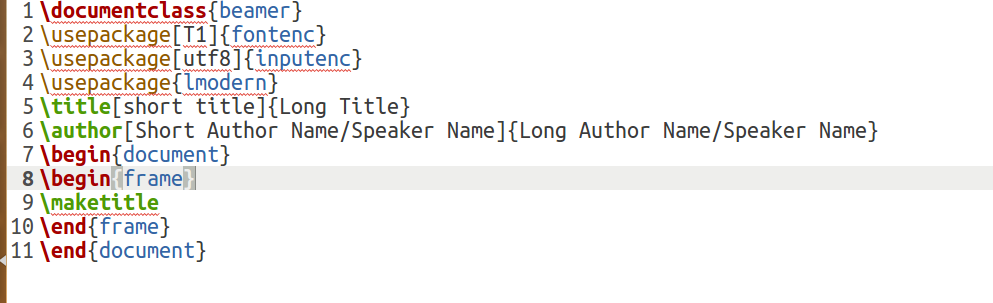
\includegraphics[width=2.5in]{figs/basic.png}
      \end{figure}
  \end{block}
\begin{block}{Output}
  \begin{figure}[ht]
    \centering
    
\includegraphics[width=2in]{figs/basic_output.png} 
  \end{figure}
    \end{block}
   \end{frame} 
%%%%%%%%%%%%%%%%%%%%%%%%%%%%%%%%%%%%%%%%%%%%%%%%%%%%%%%%%%%%%%%%%%%%%%%%%%%%%%%%%%%%%%%%%%%%%%%%%%
\subsection{}
\begin{frame}
  \frametitle{The Frame}
  A frame defines one “page” (slide) of the presentation.
  \begin{block}{Input Tex File}
\begin{figure}[ht]
    \centering
    
\includegraphics[width=2.5in]{figs/frame.png}
      \end{figure}
        \end{block}
\begin{block}{Output}
  \begin{figure}[ht]
    \centering
    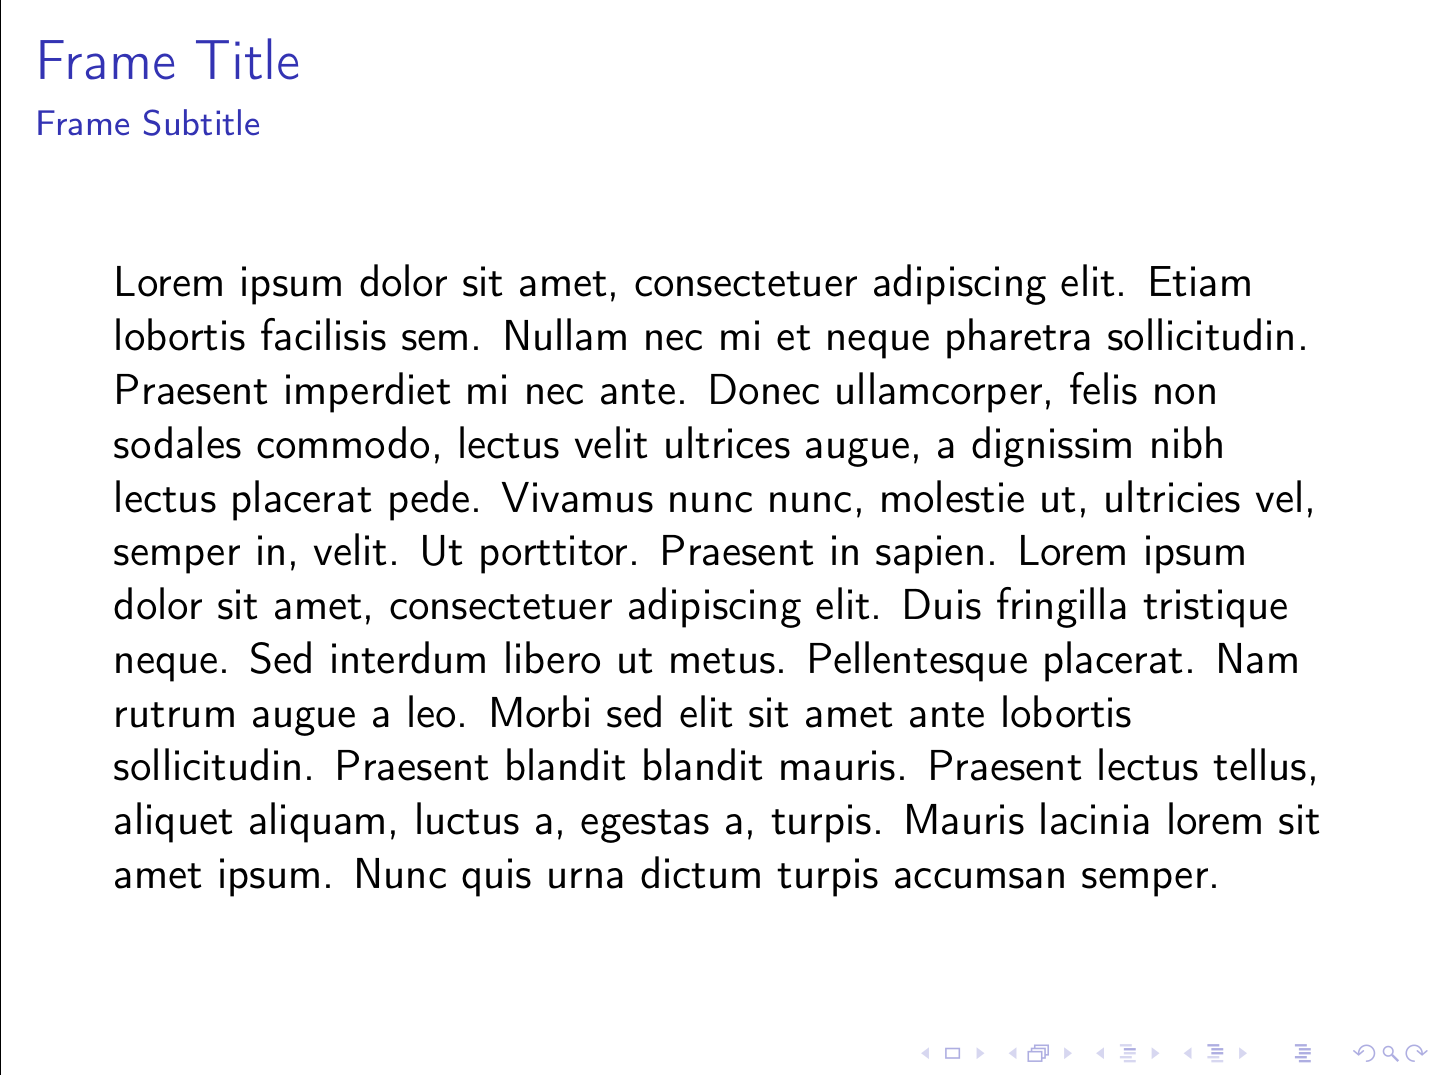
\includegraphics[width=2in]{figs/frame_output.png} 
  \end{figure}
  \end{block}
\end{frame}
%%%%%%%%%%%%%%%%%%%%%%%%%%%%%%%%%%%%%%%%%%%%%%%%%%%%%%%%%%%%%%%%%%%%%%%%%%%%%%%%%%%%%%%%%%%%%%%%%%
\section{Themes}
\subsection{}
\begin{frame}[fragile]
  \frametitle{Themes}
  \begin{small}
  For the appearance of the presentation you can select predefined \textbf{themes}
of the {\scshape Beamer} class. Thereby, {\scshape Beamer }classifies five Categories:\\
\vspace{0.67cm}
\textbf{Categories of Themes:}
\begin{enumerate}
  \item \textbf{\color{green}Presentation Themes:} slide template
  \item \textbf{\color{green} Color Themes$^*$:} color scheme of slide template
  \item \textbf{\color{green} \color{green} Font Themes$^*$:} defines the fonts
  \item \textbf{\color{green} Inner Themes$^*$:} defines inside of slide like of bullets, boxes, etc.
  \item \textbf{\color{green} Outer Themes$^*$:} defines outside of slide like head- and footlines
\end{enumerate}
($^*$ are optional, if you don’t like the default settings of Presentation themes)
  \end{small}
\end{frame}
%%%%%%%%%%%%%%%%%%%%%%%%%%%%%%%%%%%%%%%%%%%%%%%%%%%%%%%%%%%%%%%%%%%%%%%%%%%%%%%%%%%%%%%%%%%%%%%%%%
\subsection{}
\begin{frame}[fragile]
  \frametitle{Themes - Presentation Themes}
  Specifies the slide template of the entire presentation:
\begin{block}{}
\begin{verbatim}
  \usetheme[...]{Berkeley}
\end{verbatim}
\end{block}
\begin{block}{Presentation Themes (many are named after cities):}

\begin{footnotesize}
\begin{columns}
\begin{column}{.02\textwidth}
  \end{column}
  \begin{column}{.17\textwidth}
AnnArbor
Boadilla
default
Ilmenau
Marburg
Singapore
  \end{column}
  \begin{column}{.17\textwidth}
Antibes
boxes
Dresden
JuanLesPins
Montpellier
Szeged
\end{column}
\begin{column}{.17\textwidth}
Bergen\\
CambridgeUS
Frankfurt
Luebeck
PaloAlto
Warsaw
\end{column}
  \begin{column}{.17\textwidth}
Berkeley
Copenhagen
Goettingen
Madrid
Pittsburgh\\
~~~~
\end{column}
\begin{column}{.17\textwidth}
Berlin
Darmstadt
Hannover
Malmoe
Rochester\\
~~~~
\end{column}
\begin{column}{.01\textwidth}
\end{column}
\end{columns}
\end{footnotesize}
\end{block}
\end{frame}
%%%%%%%%%%%%%%%%%%%%%%%%%%%%%%%%%%%%%%%%%%%%%%%%%%%%%%%%%%%%%%%%%%%%%%%%%%%%%%%%%%%%%%%%%%%%%%%%%%
\subsection{}
\begin{frame}
  \frametitle{Using Themes}
\begin{columns}
  \begin{column}{.45\textwidth}
\begin{block}{Input Tex File}
\begin{figure}[ht]
    \centering
    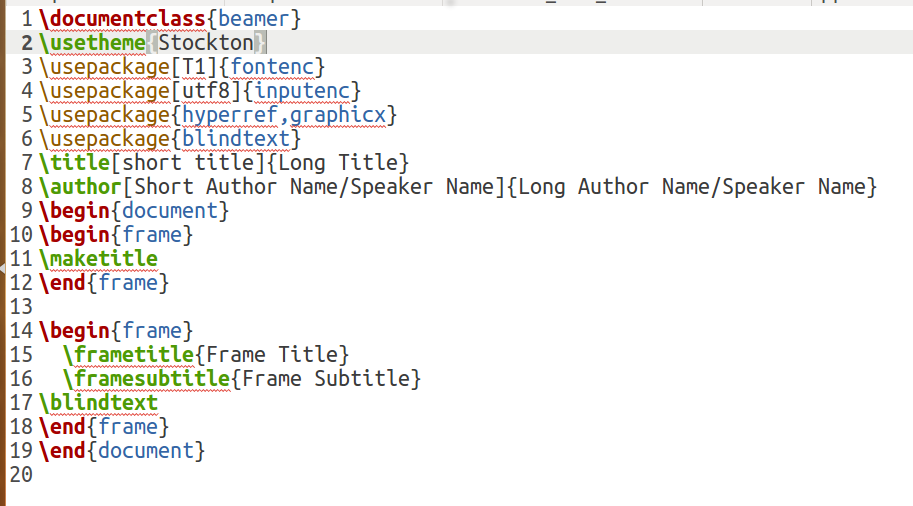
\includegraphics[width=2in,height=2.in]{figs/theme.png}
 \end{figure}
 \end{block}
  \end{column}
  \begin{column}{.55\textwidth}
\begin{block}{Output}
    \begin{figure}[ht]
    \centering
    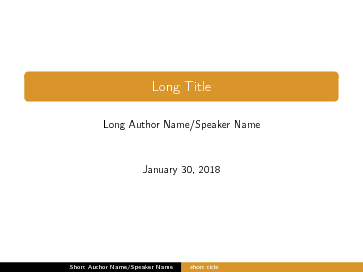
\includegraphics[width=1.75in,height=0.75in]{figs/theme-0.png}\\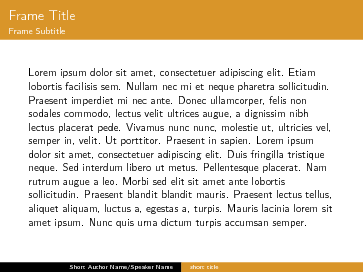
\includegraphics[width=2in]{figs/theme-1.png} 
  \end{figure}
  \end{block}
  \end{column}
\end{columns}
  \begin{small}
  \textbf{\color{green} Note:} For getting Stockton theme style file and sample latex file visit:
  \url{http://www1.pacific.edu/~smerz/Pacific_Beamer_Theme.html} 
  \end{small} 
  \end{frame}
%%%%%%%%%%%%%%%%%%%%%%%%%%%%%%%%%%%%%%%%%%%%%%%%%%%%%%%%%%%%%%%%%%%%%%%%%%%%%%%%%%%%%%%%%%%%%%%%%%
%%%%%%%%%%%%%%%%%%%%%%%%%%%%%%%%%%%%%%%%%%%%%%%%%%%%%%%%%%%%%%%%%%%%%%%%%%%%%%%%%%%%%%%%%%%%%%%%%%
\subsection{}
\begin{frame}
  \frametitle{Using Themes}
\begin{columns}
  \begin{column}{.5\textwidth}
\begin{block}{Warsaw Theme}
\begin{figure}[ht]
    \centering
    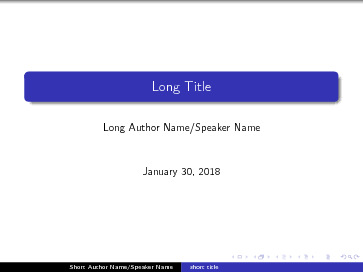
\includegraphics[width=2in,height=2.in]{figs/warsaw.png}
 \end{figure}
 \end{block}
  \end{column}
  \begin{column}{.5\textwidth}
\begin{block}{Berlin Theme}
    \begin{figure}[ht]
    \centering
    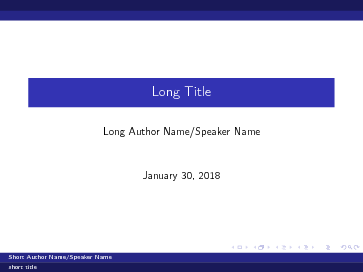
\includegraphics[width=2in,height=2in]{figs/berlin.png}
  \end{figure}
  \end{block}
  \end{column}
\end{columns}
  \end{frame}
%%%%%%%%%%%%%%%%%%%%%%%%%%%%%%%%%%%%%%%%%%%%%%%%%%%%%%%%%%%%%%%%%%%%%%%%%%%%%%%%%%%%%%%%%%%%%%%%%%%%%%%%%%%%%%%%%%%%%%%%%%%%
%%%%%%%%%%%%%%%%%%%%%%%%%%%%%%%%%%%%%%%%%%%%%%%%%%%%%%%%%%%%%%%%%%%%%%%%%%%%%%%%%%%%%%%%%%%%%%%%%%
\subsection{}
\begin{frame}
  \frametitle{Themes - Color Themes}
  Specifies the color themes of the slide template either complete or
just for inner and outer elements:
 \begin{block}{Color Themes (many are named after animals):}
   \begin{itemize}
    \item \textbf{complete:} albatross, beetle, crane, dove, fly, seagull, wolverine, beaver
    \item \textbf{ inner:} lily, orchid, rose
  \item \textbf{ outer:} whale, seahorse, dolphin
  \end{itemize}
  \end{block}
  \textbf{\color{green} Note:} Theme-Matrix presents various theme and color combinations:
\url{http://www.hartwork.org/beamer-theme-matrix/}
\end{frame}
%%%%%%%%%%%%%%%%%%%%%%%%%%%%%%%%%%%%%%%%%%%%%%%%%%%%%%%%%%%%%%%%%%%%%%%%%%%%%%%%%%%%%%%%%%%%%%%%%%
\section{Boxes}
\subsection{}
\begin{frame}[fragile=singleslide]
\begin{verbatim}
\begin{frame}
\frametitle{Colored Boxes}
  \orangebox{Theorem Orange}{If you use the orangebox 
  command, the box will be orange.}
\end{frame} 
\end{verbatim}
\frametitle{Colored Boxes}
\orangebox{Theorem Orange}{If you use the orangebox command, the box will be orange.}
\end{frame}
%%%%%%%%%%%%%%%%%%%%%%%%%%%%%%%%%%%%%%%%%%%%%%%%%%%%%%%%%%%%%%%%%%%%%%%%%%%%%%%%%%%%%%%%%%%%%%%%%%


\subsection{}
\begin{frame}
\frametitle{Colored Boxes}
\orangebox{Theorem Orange.}{If you use the orangebox command, the box will be orange.}

\greenbox{Theorem Green.}{If you use the greenbox command, the box will be green.}

\bluebox{Theorem Blue.}{If you use the bluebox command, the box will be blue.}

\graybox{Theorem Gray.}{If you use the graybox command, the box will be gray.}

\grassgreenbox{Theorem Grass Green.}{If you use the grassgreen box command, the box will be grass green.}

\end{frame}

\section{Bullets}
\subsection{}
\begin{frame}[fragile]
\frametitle{Colored Bullets}
\vspace{-.45cm}
\begin{small}
\begin{columns}
  \begin{column}{.55\textwidth}
\begin{block}{}
\begin{verbatim}
\begin{itemize}
\item These are the ordinary
\item  bullets produced
\item by the usual 
\item itemize command
\end{itemize} 
\begin{orangeitemize}
\item  \{orangeitemize\}
\item produces flat 
\item orange bullets
\end{orangeitemize}
\begin{grassgreenitemize}
\item \{grassgreenitemize\}
\item produces
\item grass green bullets
\end{grassgreenitemize}
\end{verbatim}
\end{block}
\end{column}
\begin{column}{.45\textwidth}
\begin{block}{}
\begin{itemize}
\item These are the ordinary
\item  bullets produced
\item by the usual 
\item itemize command
\end{itemize} 
\begin{orangeitemize}
\item  \{orangeitemize\}
\item produces flat 
\item orange bullets
\end{orangeitemize}
\begin{grassgreenitemize}
\item \{grassgreenitemize\} 
\item produces 
\item grass green bullets
\end{grassgreenitemize}
\end{block}
\end{column}
\end{columns}
\end{small}
\end{frame}
%%%%%%%%%%%%%%%%%%%%%%%%%%%%%%%%%%%%%%%%%%%%%%%%%%%%%%%%%%%%%%%%%%%%%%%%%%%%%%%%%%%%%%%%%%%%%%%%%%

\subsection{}
\begin{frame}[fragile]
\frametitle{Match Bullets to Box}
\grassgreenbox{Match Your Bullets}{\begin{grassgreenitemize}\item Don't forget to match \item your bullets to the box \item they live in. \end{grassgreenitemize}}
\vspace{1cm}
\orangebox{Orange Box}{\begin{orangeitemize}\item orangeitemize \item produces \item orange bullets. \end{orangeitemize}}
\end{frame}
%%%%%%%%%%%%%%%%%%%%%%%%%%%%%%%%%%%%%%%%%%%%%%%%%%%%%%%%%%%%%%%%%%%%%%%%%%%%%%%%%%%%%%%%%%%%%%%%%%
\subsection{}
\begin{frame}
  \frametitle{Environments - Lists}
  $\Longrightarrow$ Usual \LaTeX~ environments are available
  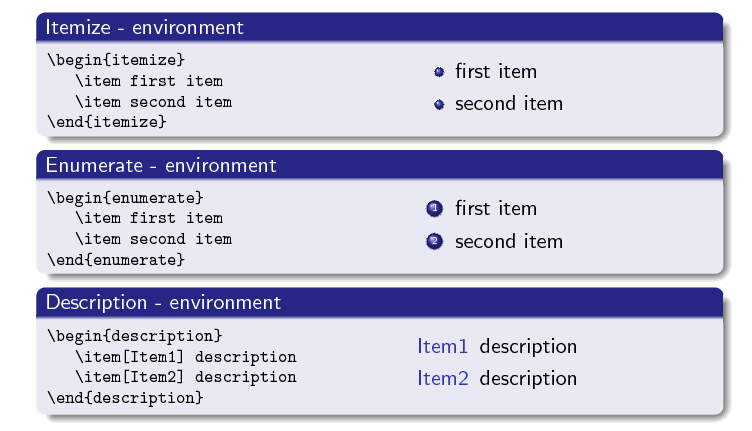
\includegraphics[width=4.25in,height=2.25in]{figs/envi}
\end{frame}
%%%%%%%%%%%%%%%%%%%%%%%%%%%%%%%%%%%%%%%%%%%%%%%%%%%%%%%%%%%%%%%%%%%%%%%%%%%%%%%%%%%%%%%%%%%%%%%%%%
\section{Overlays}
\subsection{}
\begin{frame}[fragile]
  \frametitle{Overlays - Pause}
  \vspace{-.4cm}
  \begin{block}{Pause command}
  An easy way to create overlays is the \verb+\pause+ command.
If you use this command somewhere in the frame, only the text on the
frame up to the \verb+\pause+ command is shown on the first slide. On the
second slide, everything up to the second \verb+\pause+, and so forth.
  \end{block}
\begin{small}
\begin{minipage}{.475\textwidth}
\begin{enumerate}
\item Shown from first slide on.
\pause
\item Shown from second slide on.
\pause
\item Shown from third slide on.
\pause
\item Shown from fourth slide on.
\pause
\end{enumerate}
\end{minipage}%
\hfill
\begin{minipage}{.5\textwidth}
~
\begin{verbatim}
\begin{enumerate}
\item Shown from first slide on.
\pause
\item Shown from second slide on.
\pause
\item Shown from third slide on.
\pause
\item Shown from fourth slide on.
\end{enumerate}
\end{verbatim}
\end{minipage}

~\\
$\Rightarrow $ Can be used inside environments, mathematical equation \& texts.
\end{small}
\end{frame}
%%%%%%%%%%%%%%%%%%%%%%%%%%%%%%%%%%%%%%%%%%%%%%%%%%%%%%%%%%%%%%%%%%%%%%%%%%%%%%%%%%%%%%%%%%%%%%%%%%
%%%%%%%%%%%%%%%%%%%%%%%%%%%%%%%%%%%%%%%%%%%%%%%%%%%%%%%%%%%%%%%%%%%%%%%%%%%%%%%%%%%%%%%%%%%%%%%%%%
\subsection{}
\begin{frame}[fragile]
  \frametitle{Overlays - Specifications}
 \begin{itemize}
   \item Overlays specifications are given in pointed brackets <...>  which can be written behind certain commands.
\item These specifications indicate which slide the corresponding information should appear on, as explained in the following:
\item $ <2> \;\rightarrow$ display on slide 2.
\item $< 1-> \; \rightarrow$ display from slide 1 on.
\item $<1-3>\; \rightarrow$ display from slide 1 to slide 3.
\item $<-3, 5-6, 8->\; \rightarrow$ display on all slides except slides 4 and 7.
 \end{itemize}
\begin{block}{}
\begin{minipage}{.45\textwidth}
\begin{small}
\begin{itemize}
\item<1-> Shown from first slide on.
\item<2-> Shown from second slide on.
\item<4> Shown only in forth slide.
\item<3,5-> Shown in 3., 5. and all
further slides.
\end{itemize}
\end{small}
\end{minipage}%
\hfill
\begin{minipage}{.55\textwidth}
~
\begin{footnotesize}
\begin{verbatim}
\begin{itemize}
\item<1-> Shown from first slide on.
\item<2-> Shown from second slide on.
\item<4> Shown only in forth slide.
\item<3,5-> Shown in 3., 5. and all
further slides.
\end{itemize}
\end{verbatim}
\end{footnotesize}
\end{minipage}

\end{block}
\end{frame}
%%%%%%%%%%%%%%%%%%%%%%%%%%%%%%%%%%%%%%%%%%%%%%%%%%%%%%%%%%%%%%%%%%%%%%%%%%%%%%%%%%%%%%%%%%%%%%%%%%
\subsection{}
\begin{frame}[fragile]
  \frametitle{Overlays Specifications - Example}
\begin{block}{Input Tex}
\begin{verbatim}
\alert{Alert on all slides.}\\
\alert<2>{Alert on slide 2}\\
\alert<3>{Alert on slide 3}\\
\alert<1,3>{Alert on slides 1 and 3}\\
\alert<-2,4>{Alert on slides 1,2 and 4}\\
\end{verbatim}
 \end{block}
\begin{block}{Output}
\alert{Alert on all slides.}\\
\alert<2>{Alert on slide 2}\\
\alert<3>{Alert on slide 3}\\
\alert<1,3>{Alert on slides 1 and 3}\\
\alert<-2,4>{Alert on slides 1,2 and 4}\\
 \end{block}
\end{frame}
%%%%%%%%%%%%%%%%%%%%%%%%%%%%%%%%%%%%%%%%%%%%%%%%%%%%%%%%%%%%%%%%%%%%%%%%%%%%%%%%%%%%%%%%%%%%%%%%%%
\section{Graphics}
\subsection{}
\begin{frame}[fragile]
\frametitle{Including Graphics}
\begin{itemize}
  \item Standard \LaTeX~ figure environment can be used
  \item →\verb+\includegraphics[options]{filename}+
\end{itemize}
\textbf{Options are:}\\
\begin{itemize}
\item scale=<value>: scale the picture by <value>
\item height=<len>: scale the picture so that the width is <len>
\item width=<len>: scale the picture so that the width is <len>
\item angle=<x>: rotate the picture by <x> degrees
\item draft: Don’t display image, print filename in a box of the same size.
\end{itemize}
\end{frame}
%%%%%%%%%%%%%%%%%%%%%%%%%%%%%%%%%%%%%%%%%%%%%%%%%%%%%%%%%%%%%%%%%%%%%%%%%%%%%%%%%%%%%%%%%%%%%%%%%%
\subsection{}
\begin{frame}[fragile]
\frametitle{Including Graphics}
\only<1>{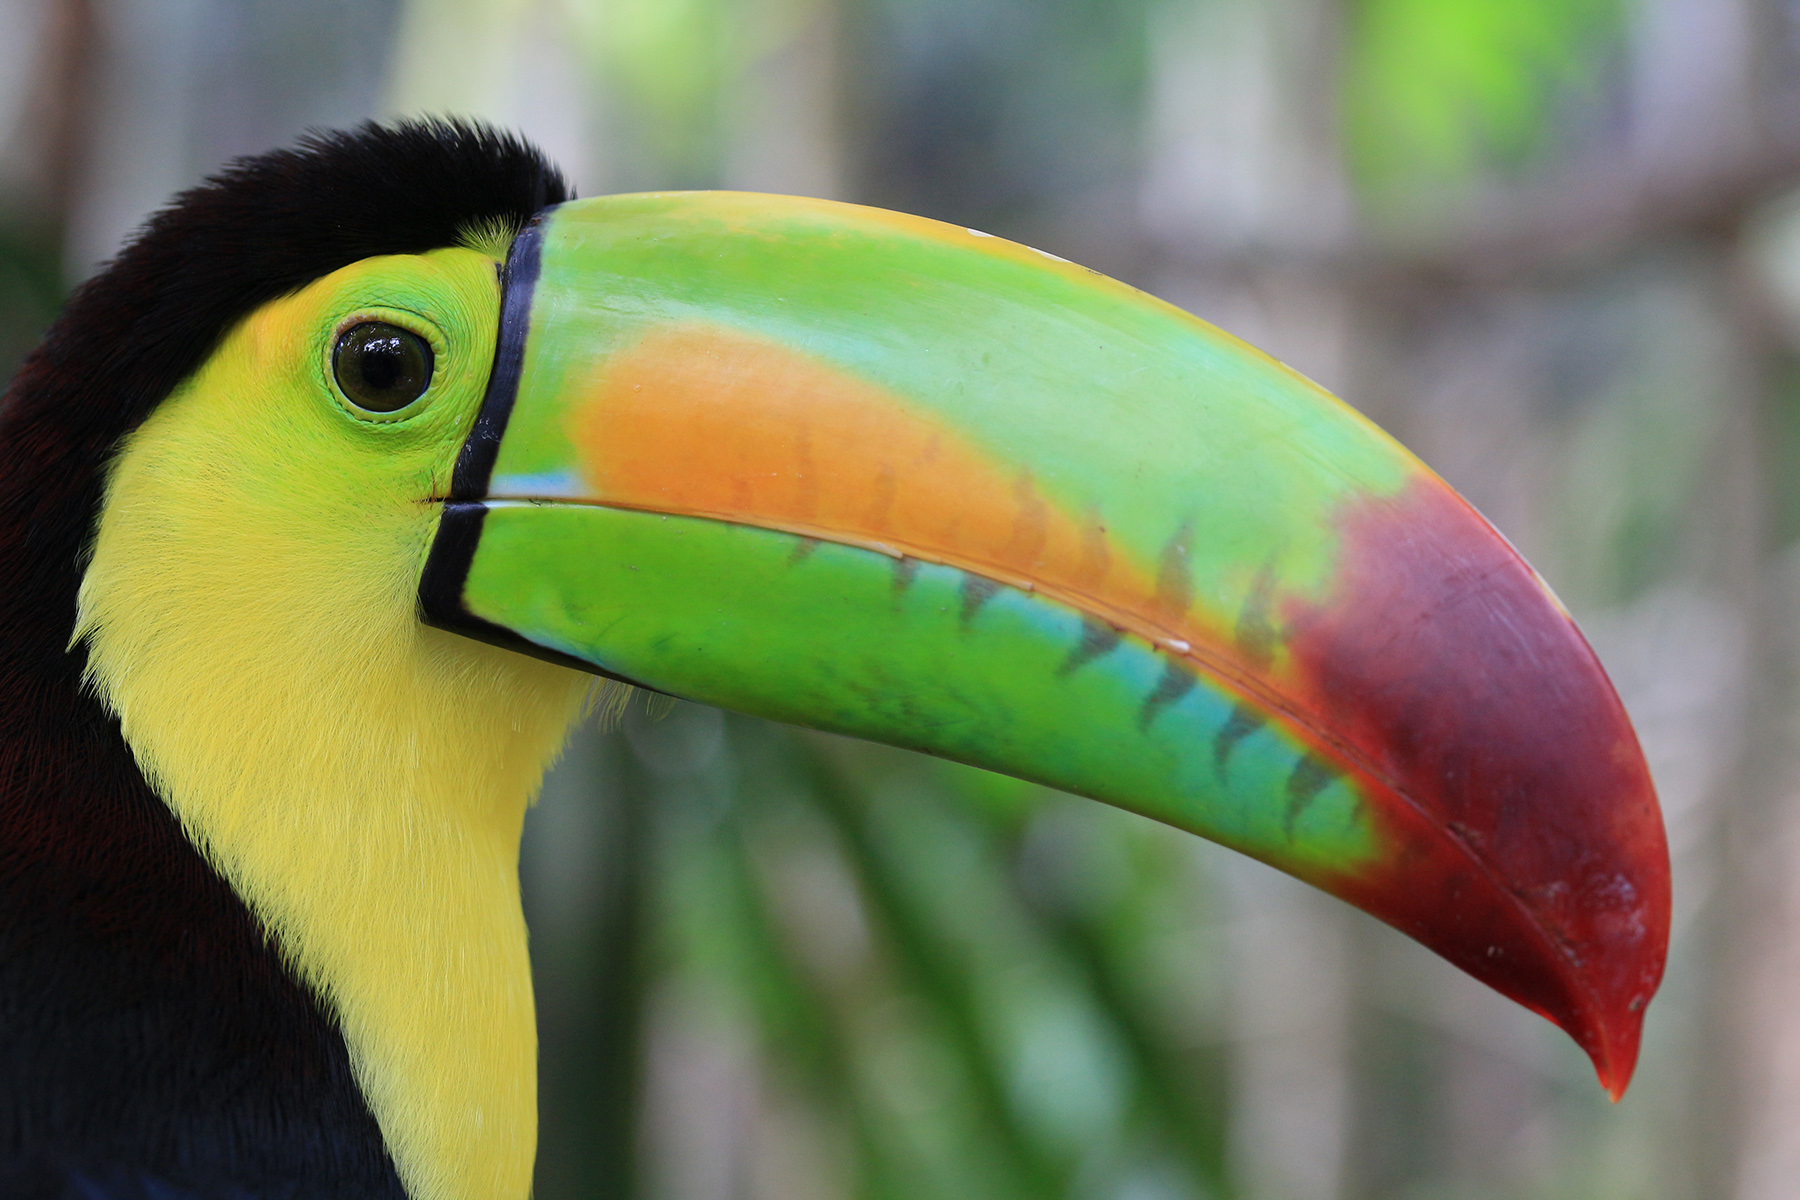
\includegraphics{figs/sample1}}
\only<2>{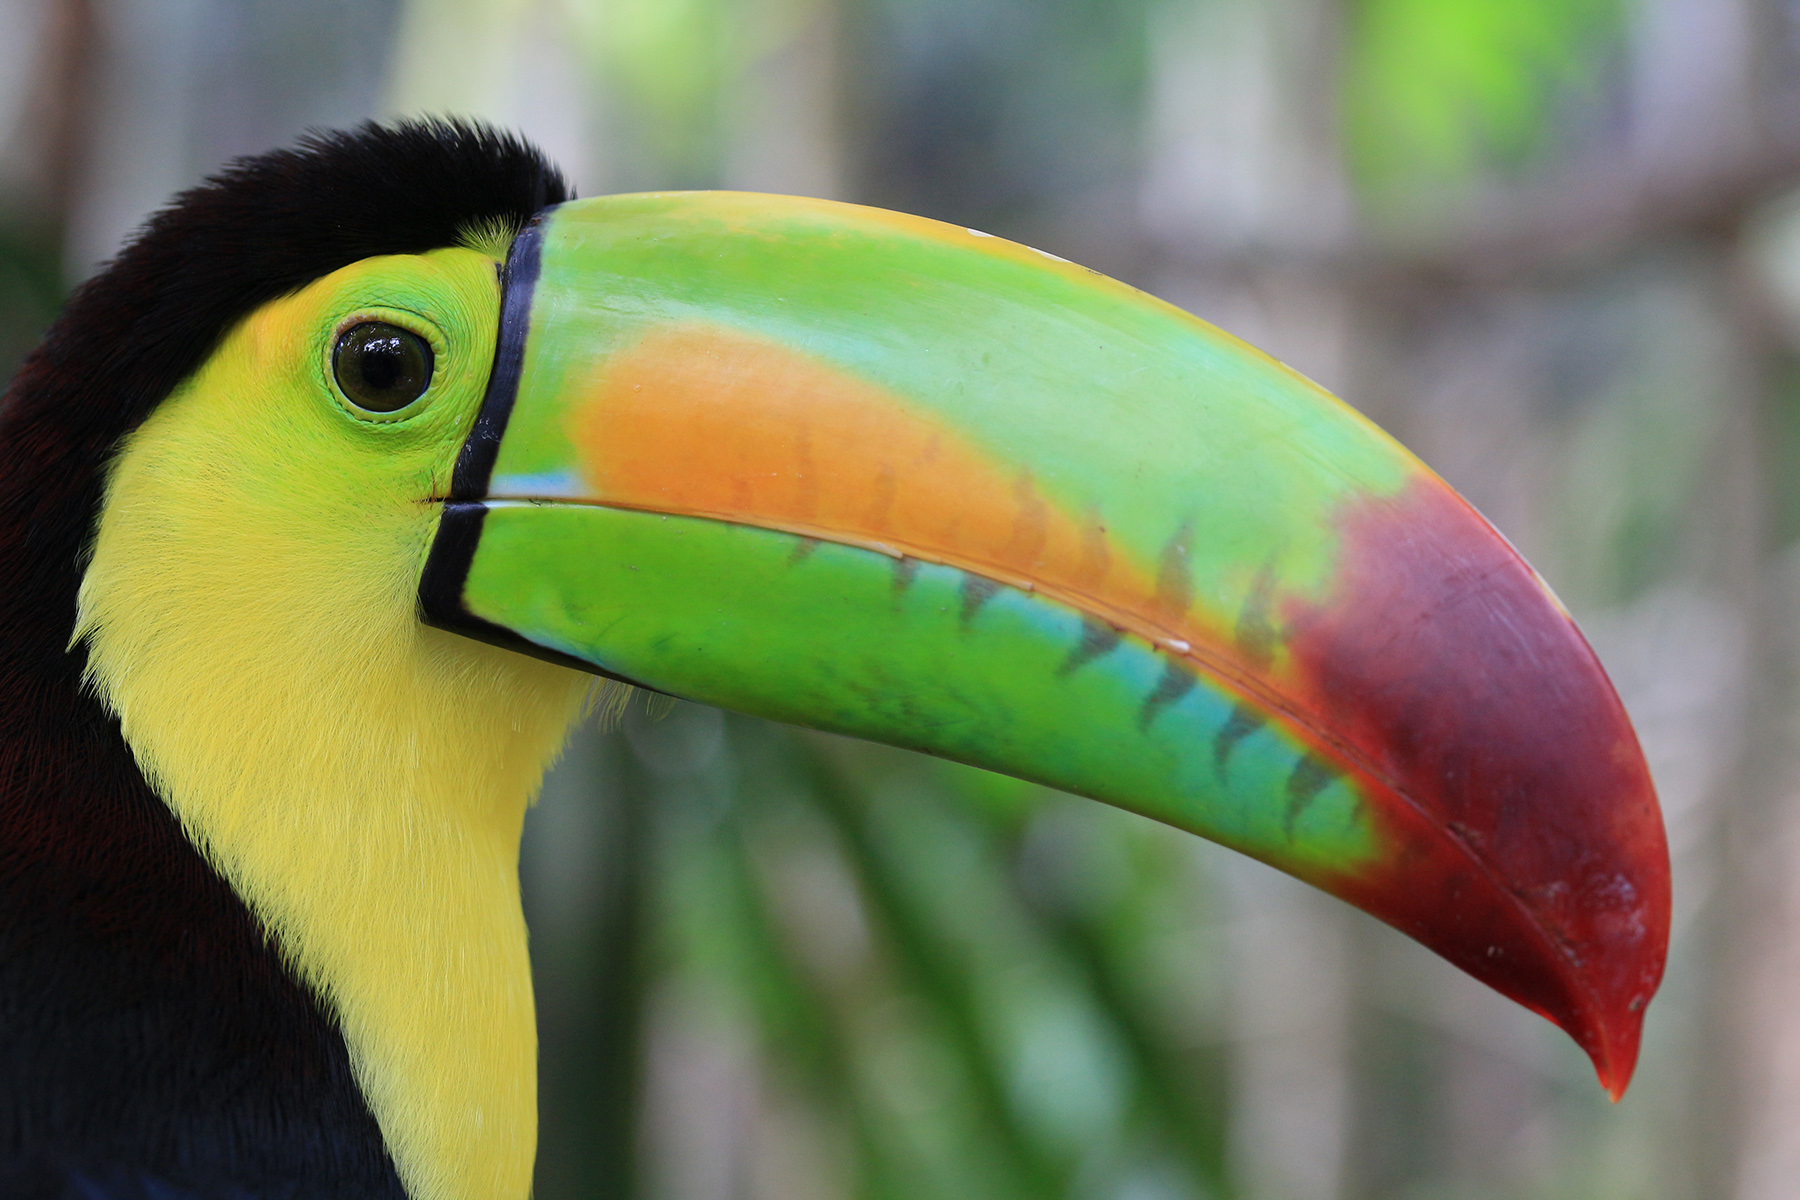
\includegraphics[scale=0.15]{figs/sample1}\\\begin{center}
\textbf{scale=0.15}
\end{center}}
\only<3>{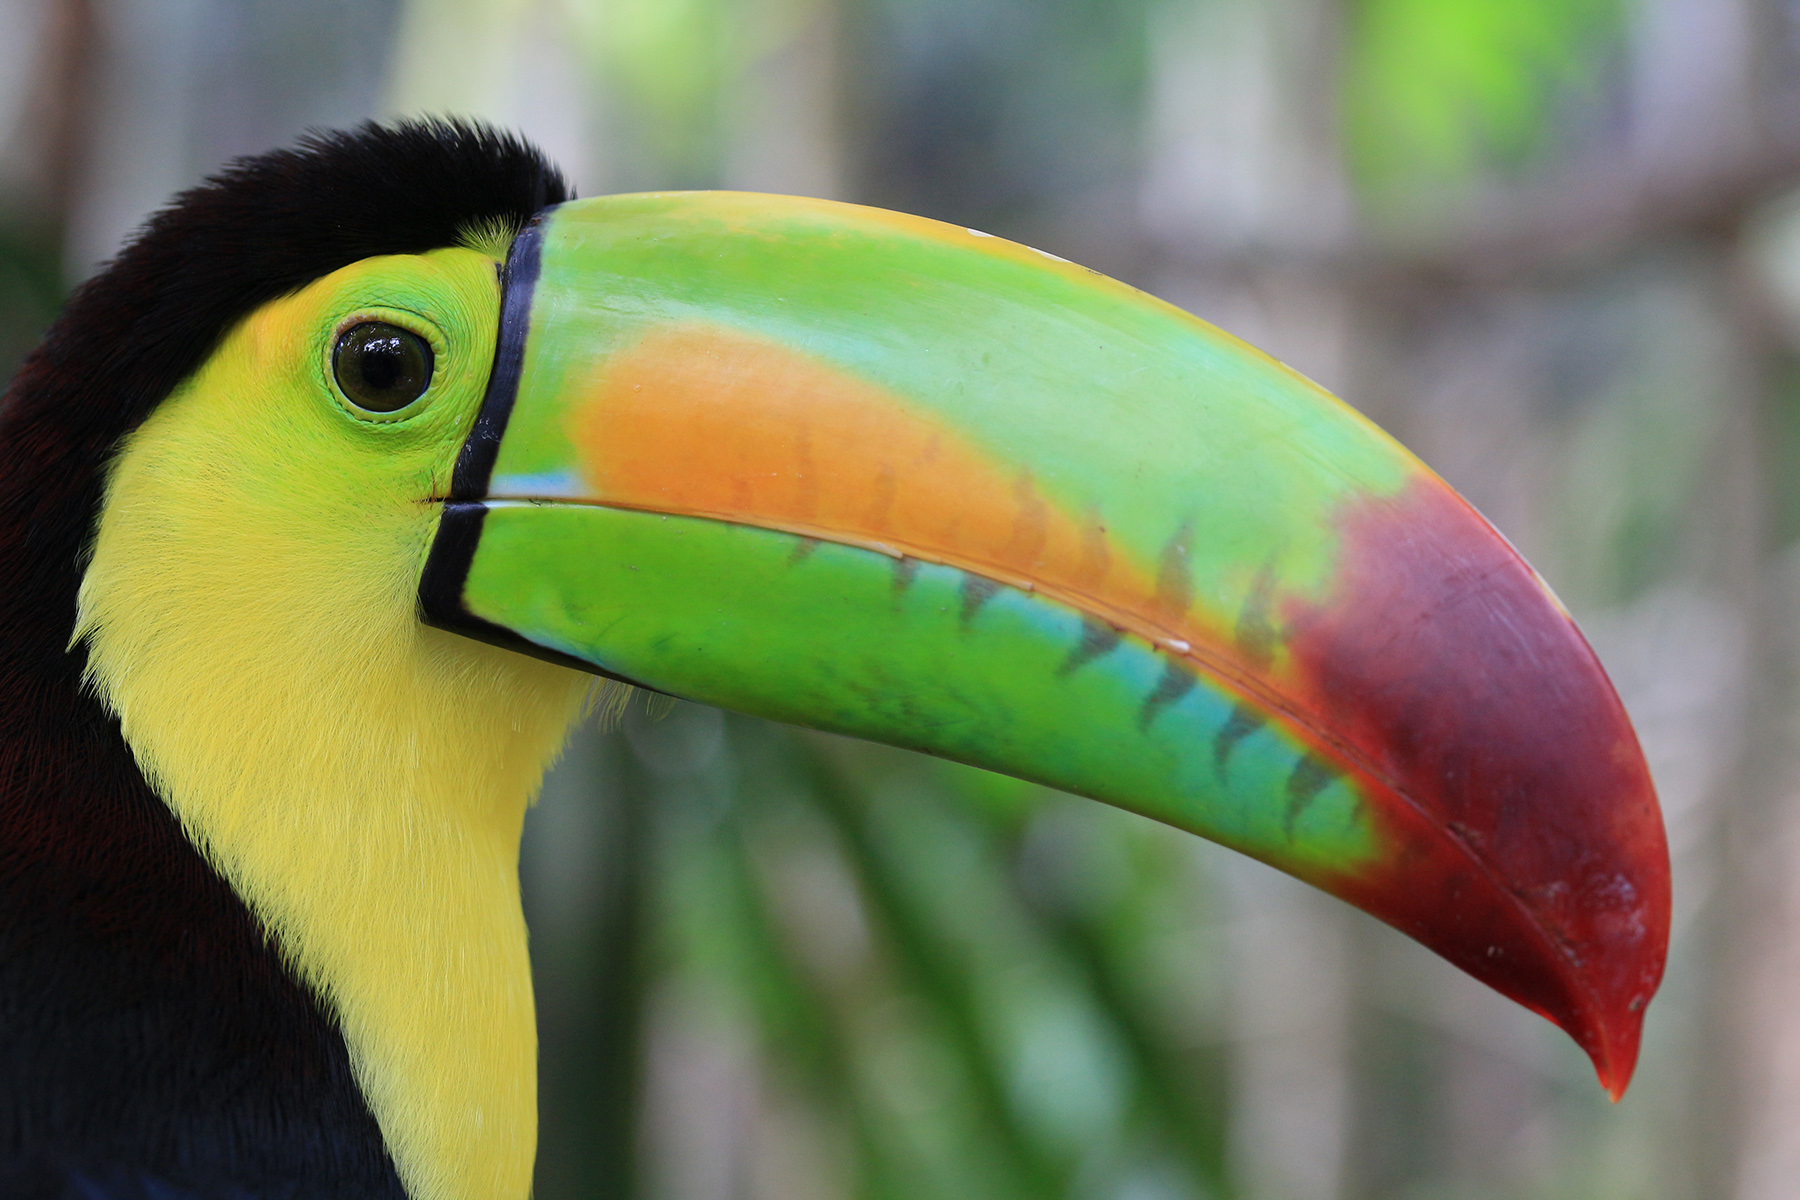
\includegraphics[height=1.5in]{figs/sample1}\\\begin{center}
\textbf{height=1.5in}
\end{center}}
\only<4>{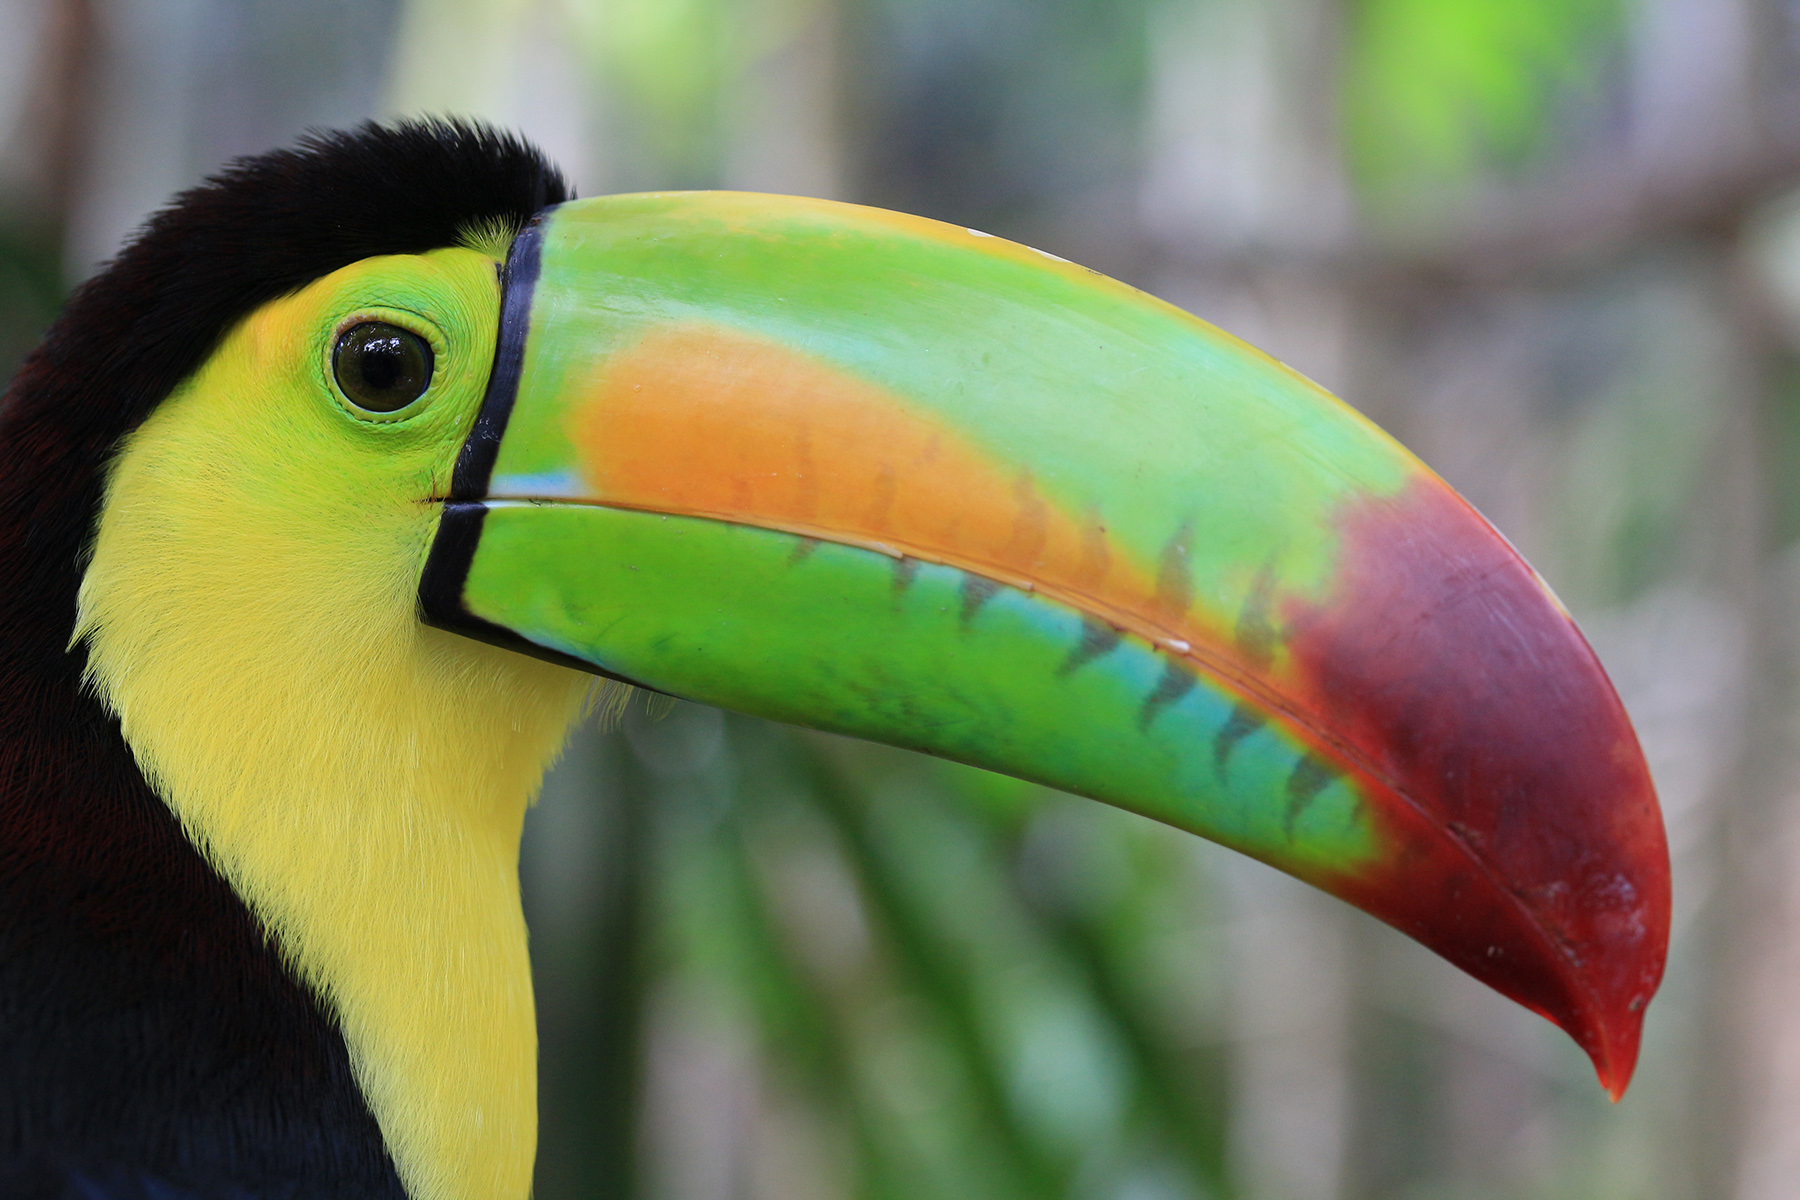
\includegraphics[width=3in]{figs/sample1}\\\begin{center}
\textbf{width=3in}
\end{center}}
\only<5>{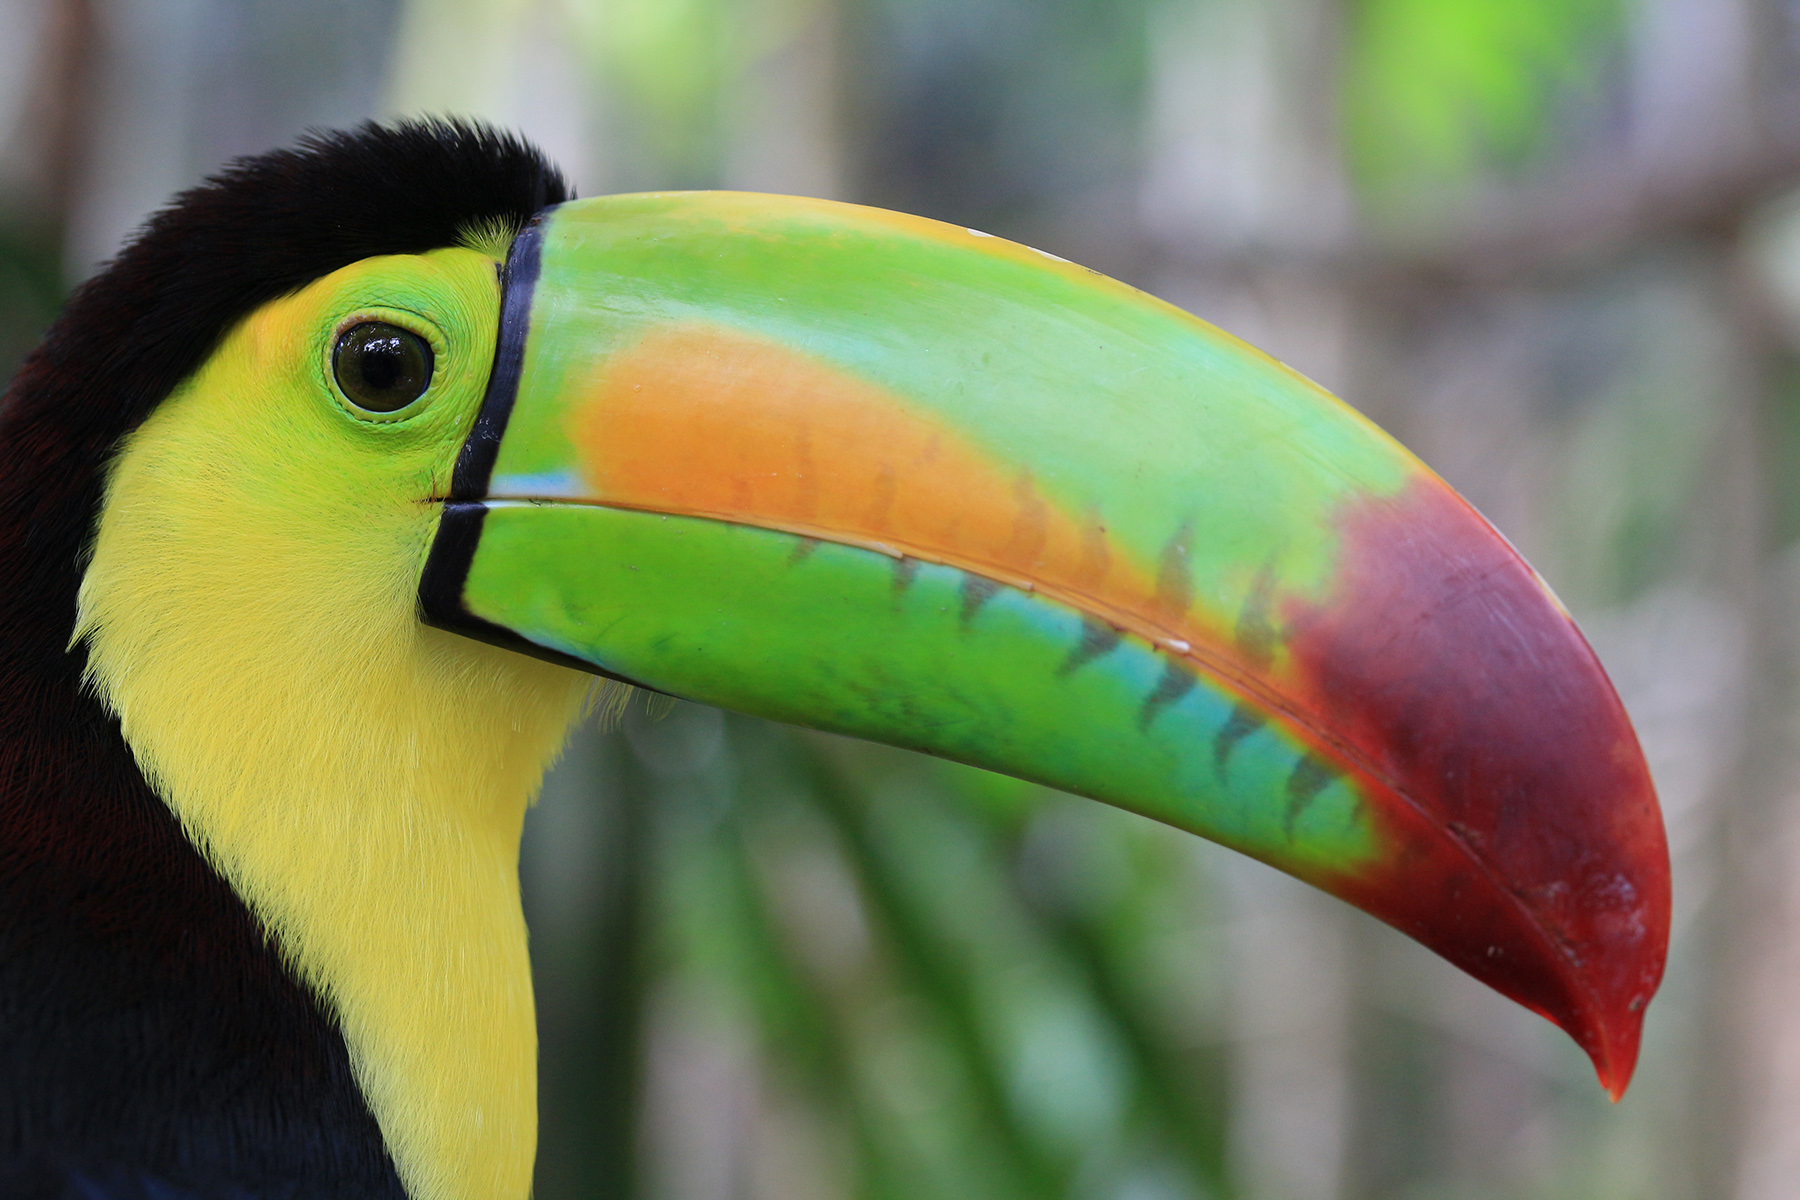
\includegraphics[height=2.5in,width=3.5in]{figs/sample1}\\\begin{center}
\textbf{ height=2.5in,width=3.5in}
\end{center}}
\only<6>{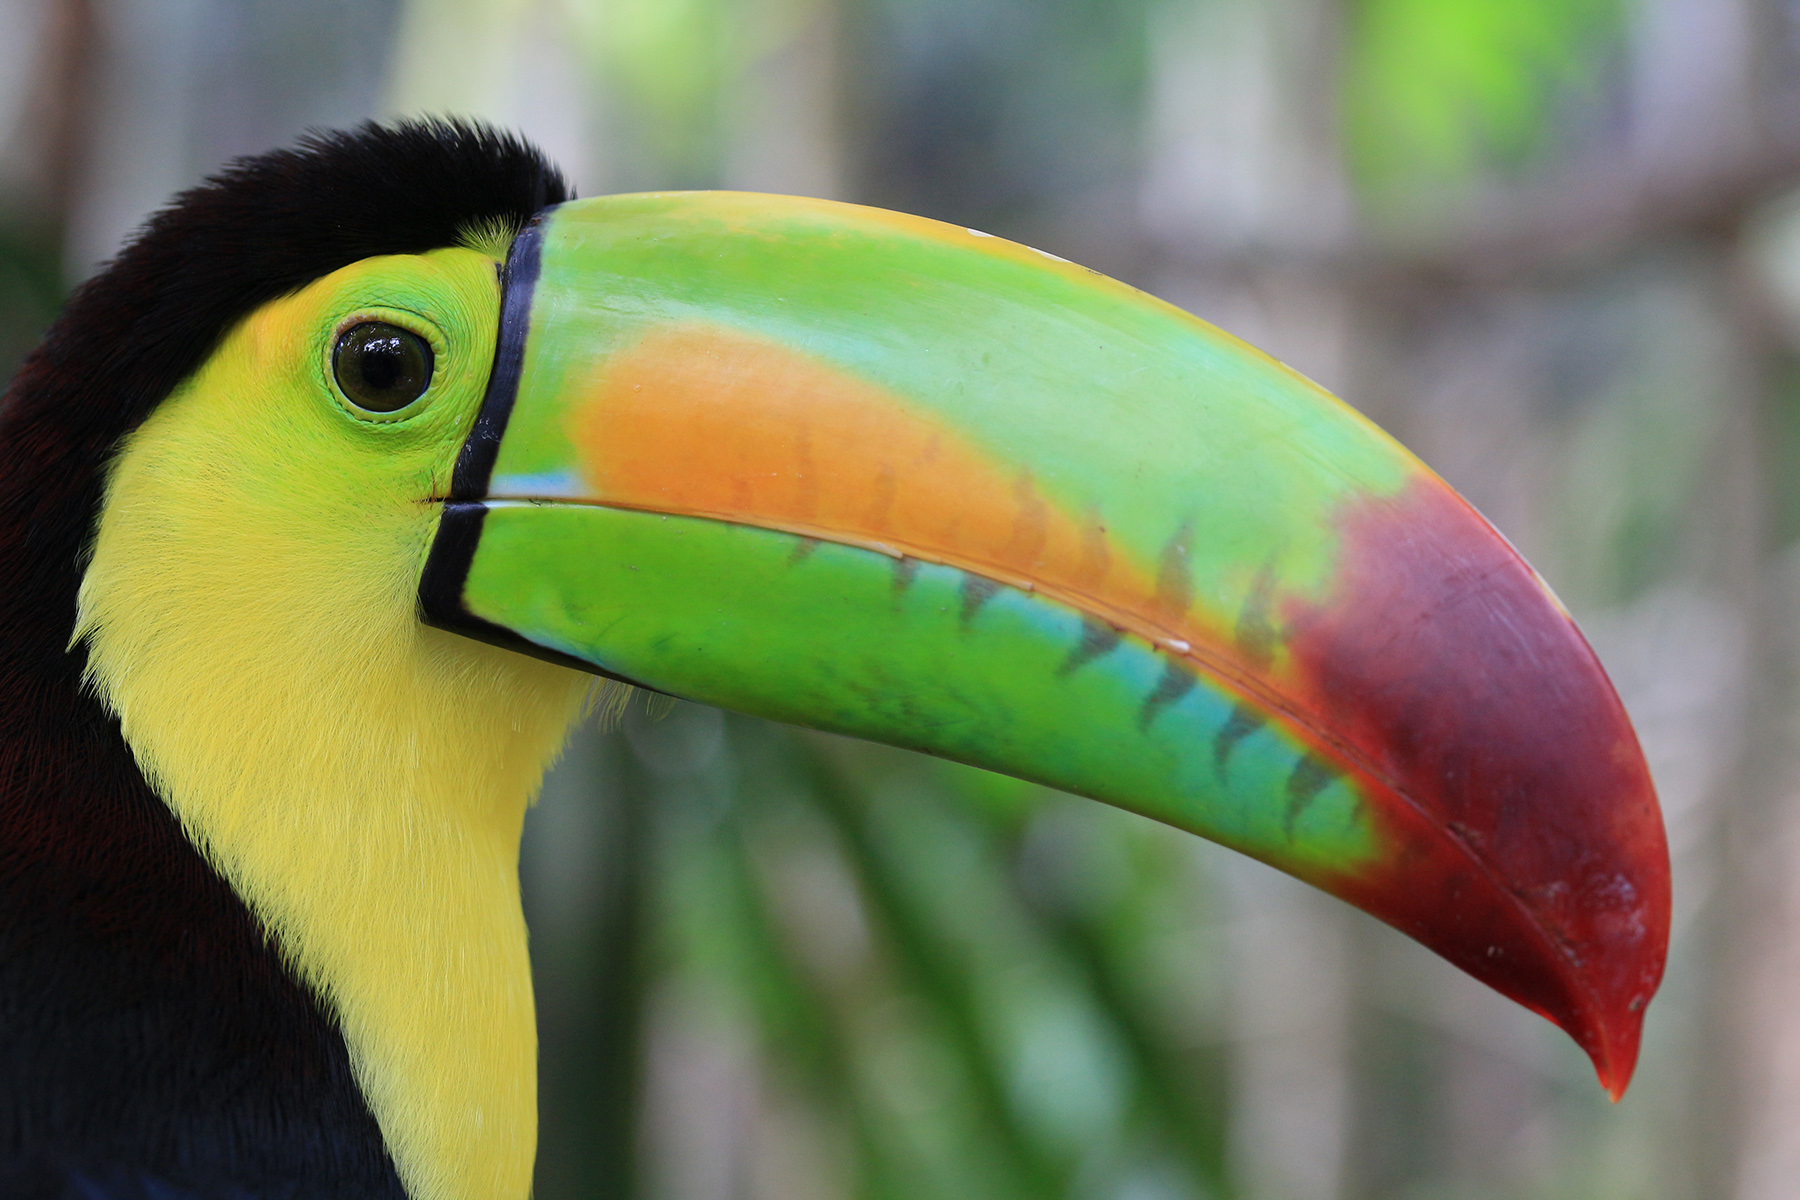
\includegraphics[angle=90,height=2.5in,width=3.5in]{figs/sample1}\\\begin{center}
\textbf{angle=90,height=2.5in,width=3.5in}\end{center}}
\only<7>{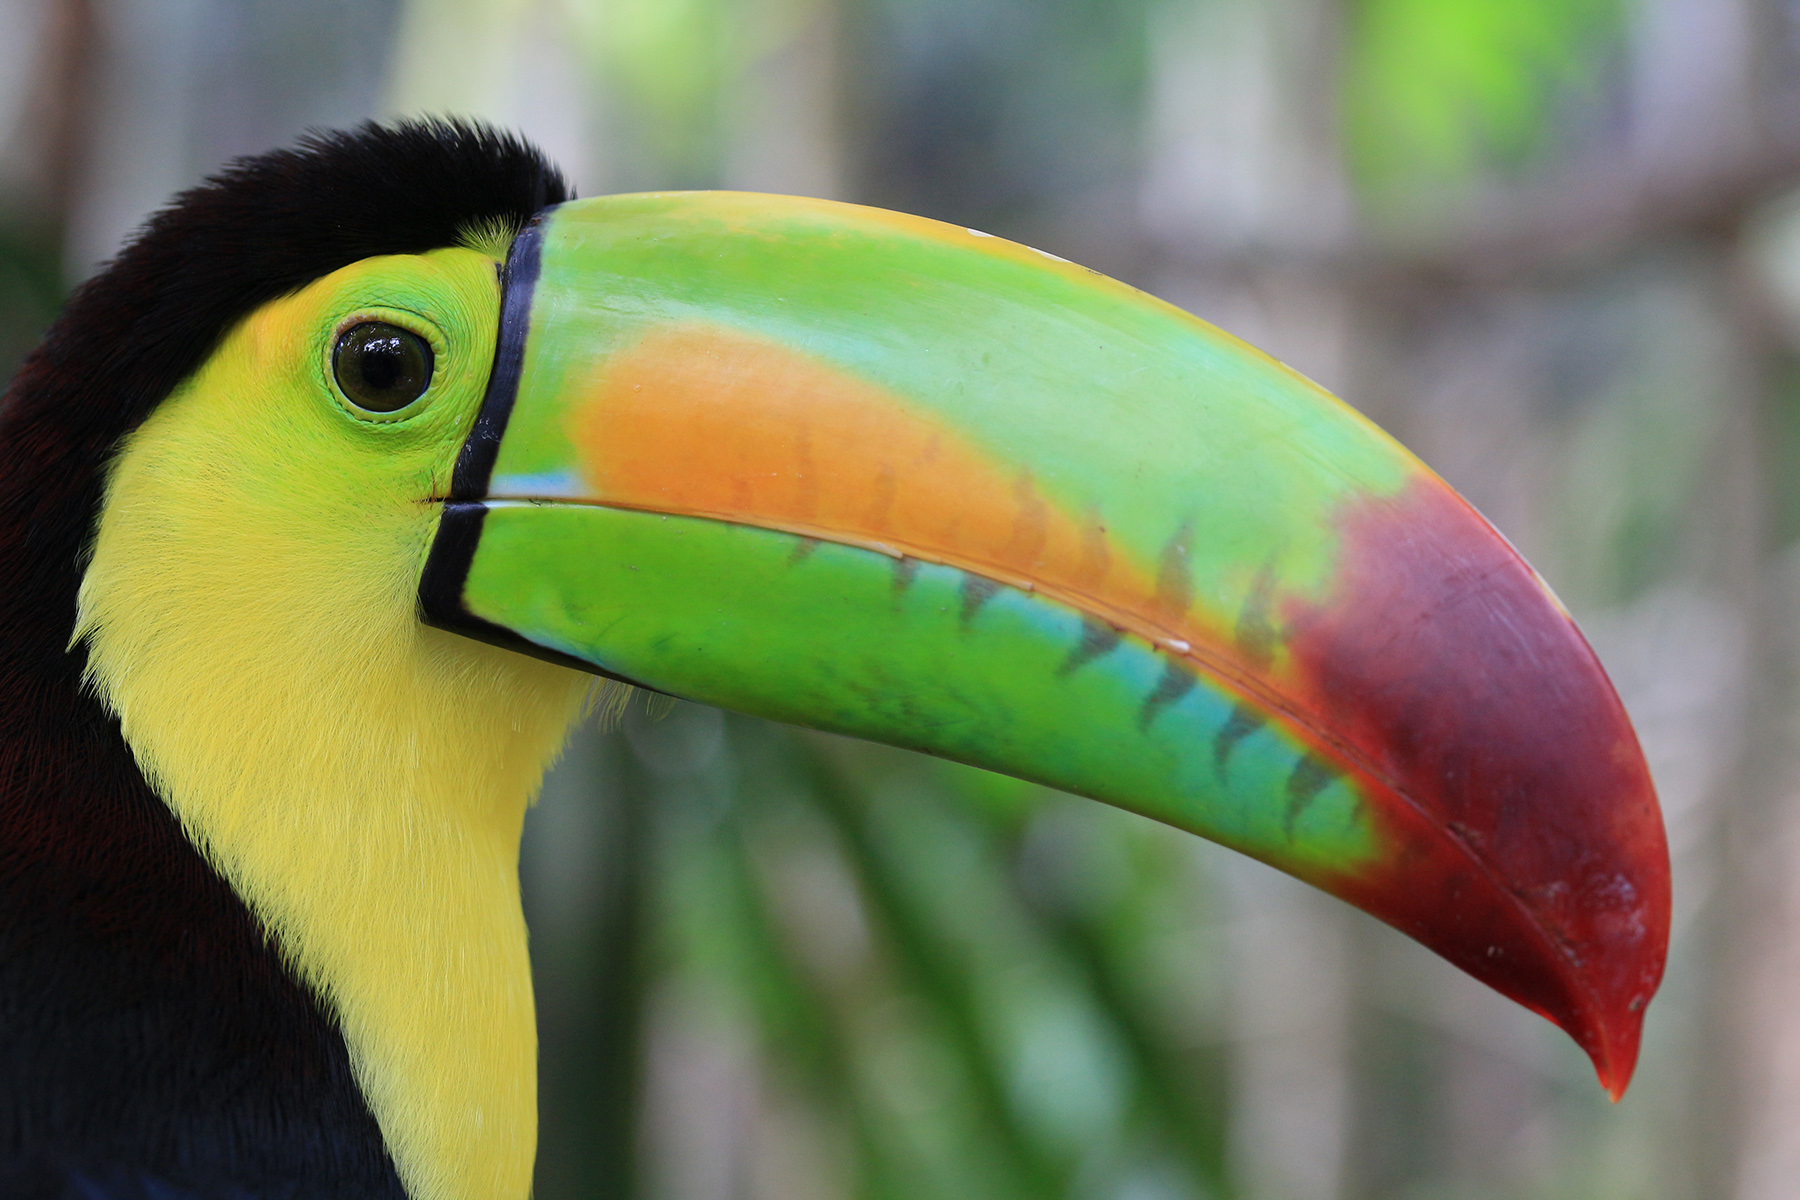
\includegraphics[draft,height=2.5in,width=3.5in]{figs/sample1}\\\begin{center}
\textbf{draft,height=2.5in,width=3.5in}\end{center}}
\end{frame}
%%%%%%%%%%%%%%%%%%%%%%%%%%%%%%%%%%%%%%%%%%%%%%%%%%%%%%%%%%%%%%%%%%%%%%%%%%%%%%%%%%%%%%%%%%%%%%%%%%
%%%%%%%%%%%%%%%%%%%%%%%%%%%%%%%%%%%%%%%%%%%%%%%%%%%%%%%%%%%%%%%%%%%%%%%%%%%%%%%%%%%%%%%%%%%%%%%%%%
\subsection{}
\begin{frame}[fragile]
  \frametitle{Including Graphics}
  \framesubtitle{Subfigures}
  \begin{tiny}
  \begin{verbatim}
\begin{figure}
    \centering
    \begin{subfigure}[b]{0.3\textwidth}
        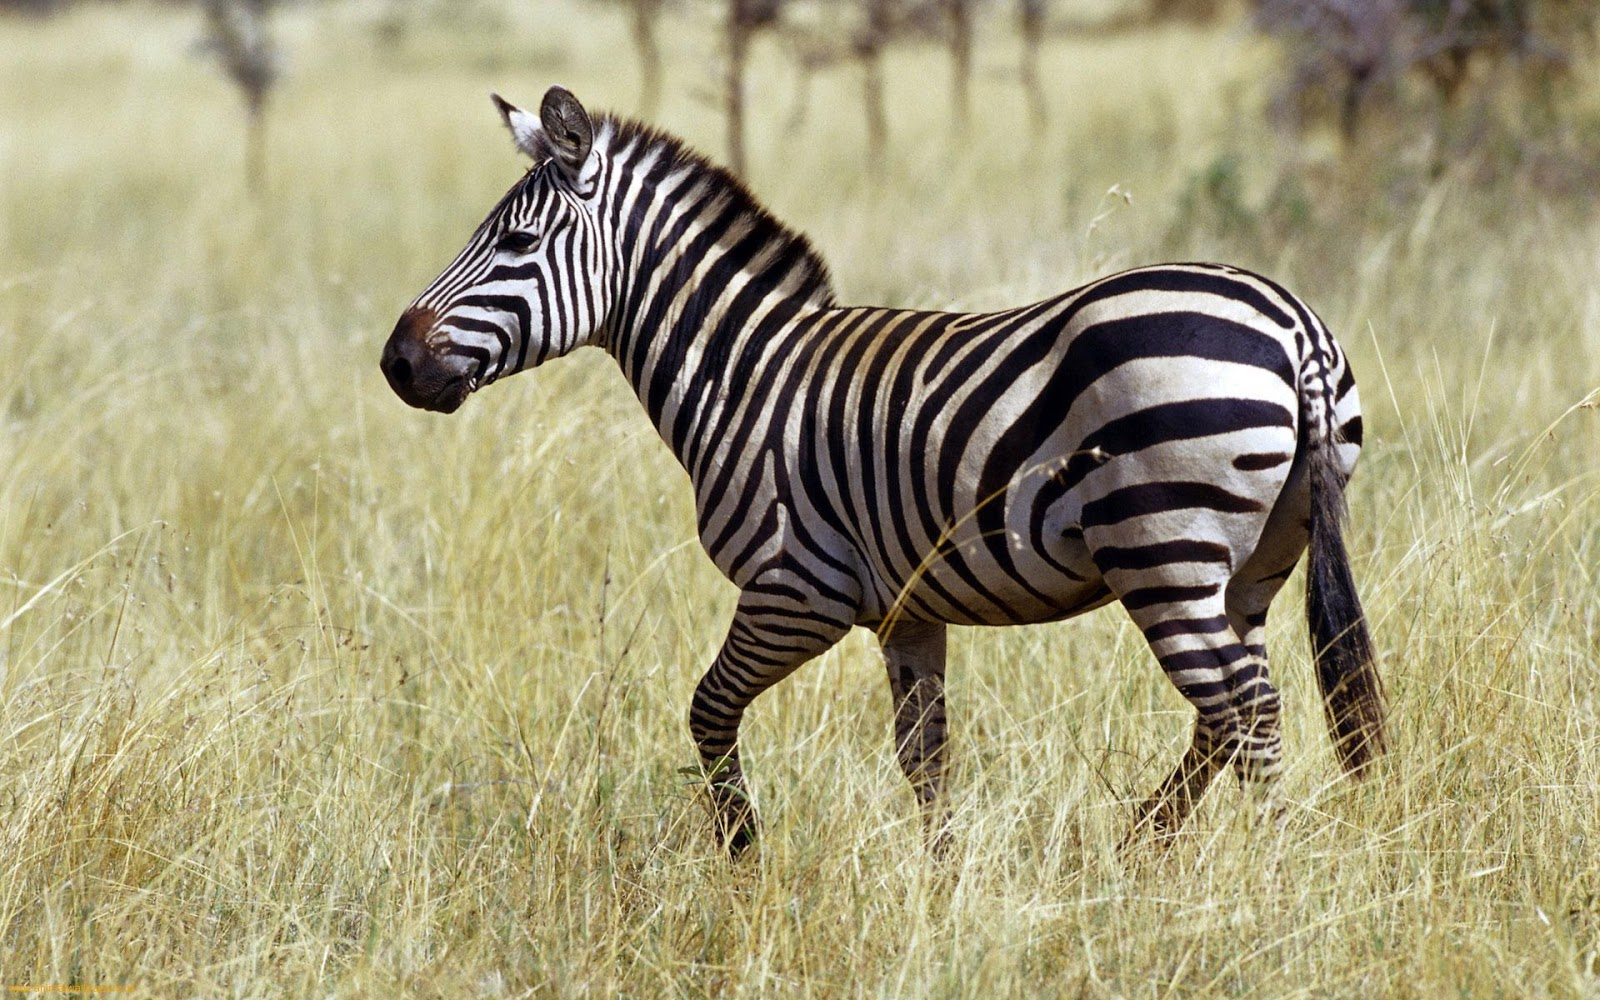
\includegraphics[width=\textwidth,height=1in]{figs/animal1}
        \caption{A Zebra}
        \label{fig:Zebra}
    \end{subfigure}
       \begin{subfigure}[b]{0.3\textwidth}
        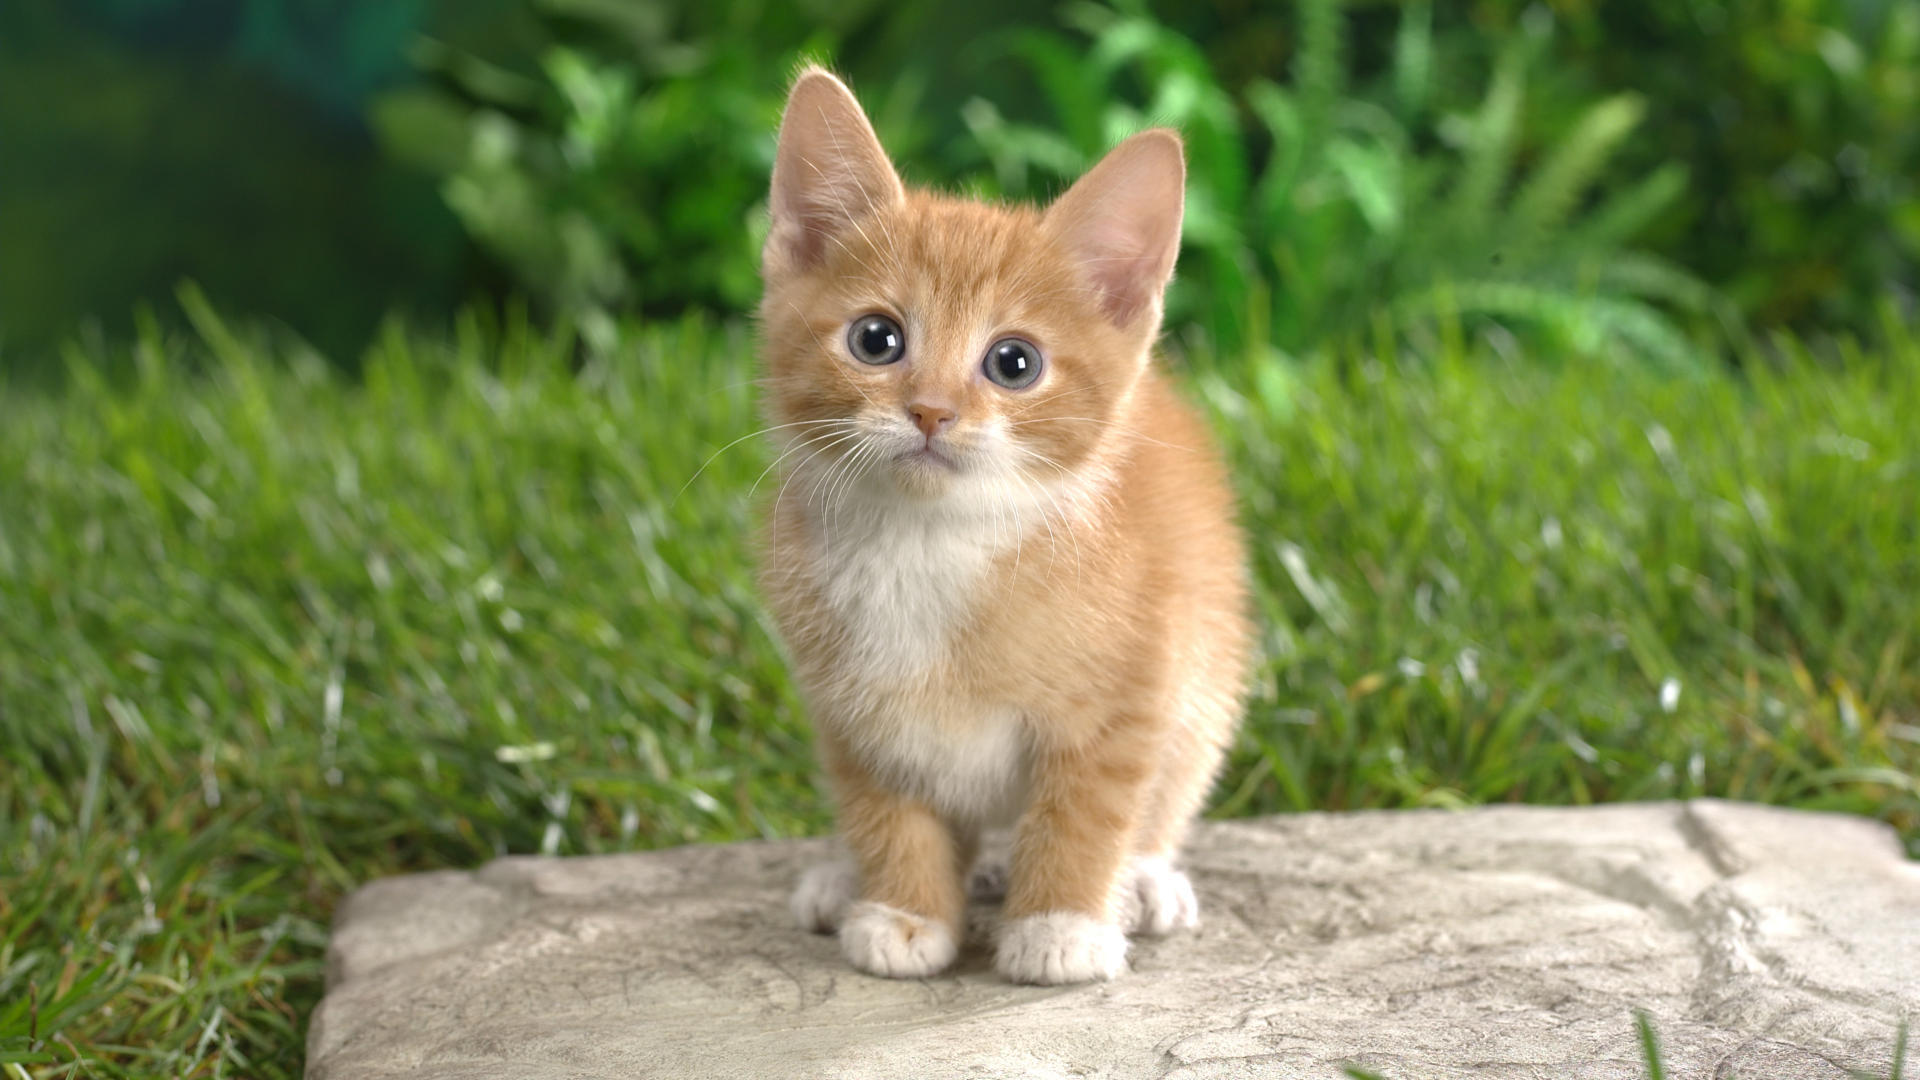
\includegraphics[width=\textwidth,height=1in]{figs/animal2}
        \caption{A Cat}
        \label{fig:cat}
    \end{subfigure}
       \begin{subfigure}[b]{0.3\textwidth}
        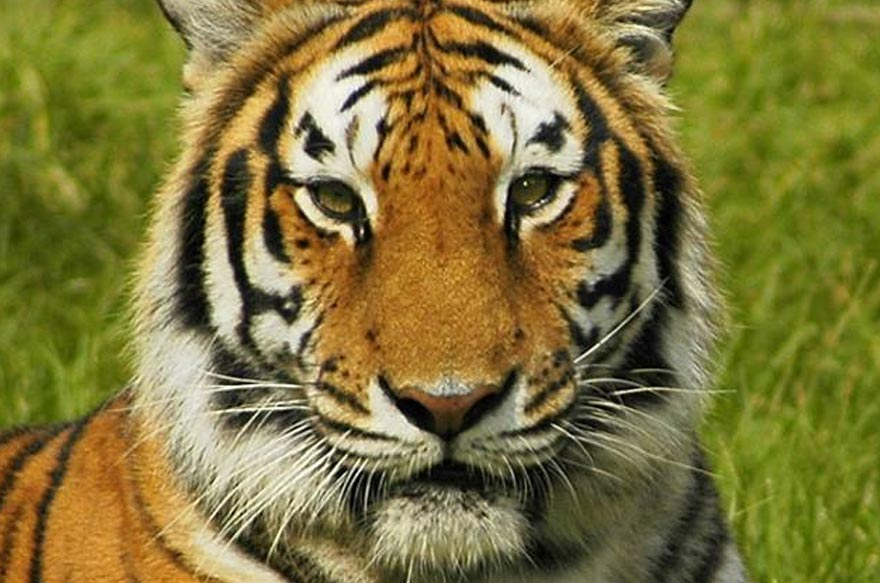
\includegraphics[width=\textwidth,height=1in]{figs/animal3}
        \caption{A Tiger}
        \label{fig:tiger}
    \end{subfigure}
    \caption{Pictures of animals}\label{fig:animals}
\end{figure}
\end{verbatim}
  \end{tiny}
\end{frame}
%%%%%%%%%%%%%%%%%%%%%%%%%%%%%%%%%%%%%%%%%%%%%%%%%%%%%%%%%%%%%%%%%%%%%%%%%%%%%%%%%%%%%%%%%%%%%%%%%%
\subsection{}
\begin{frame}
  \frametitle{Including Graphics}
  \framesubtitle{Subfigures}
\begin{figure}
    \centering
    \begin{subfigure}[b]{0.3\textwidth}
        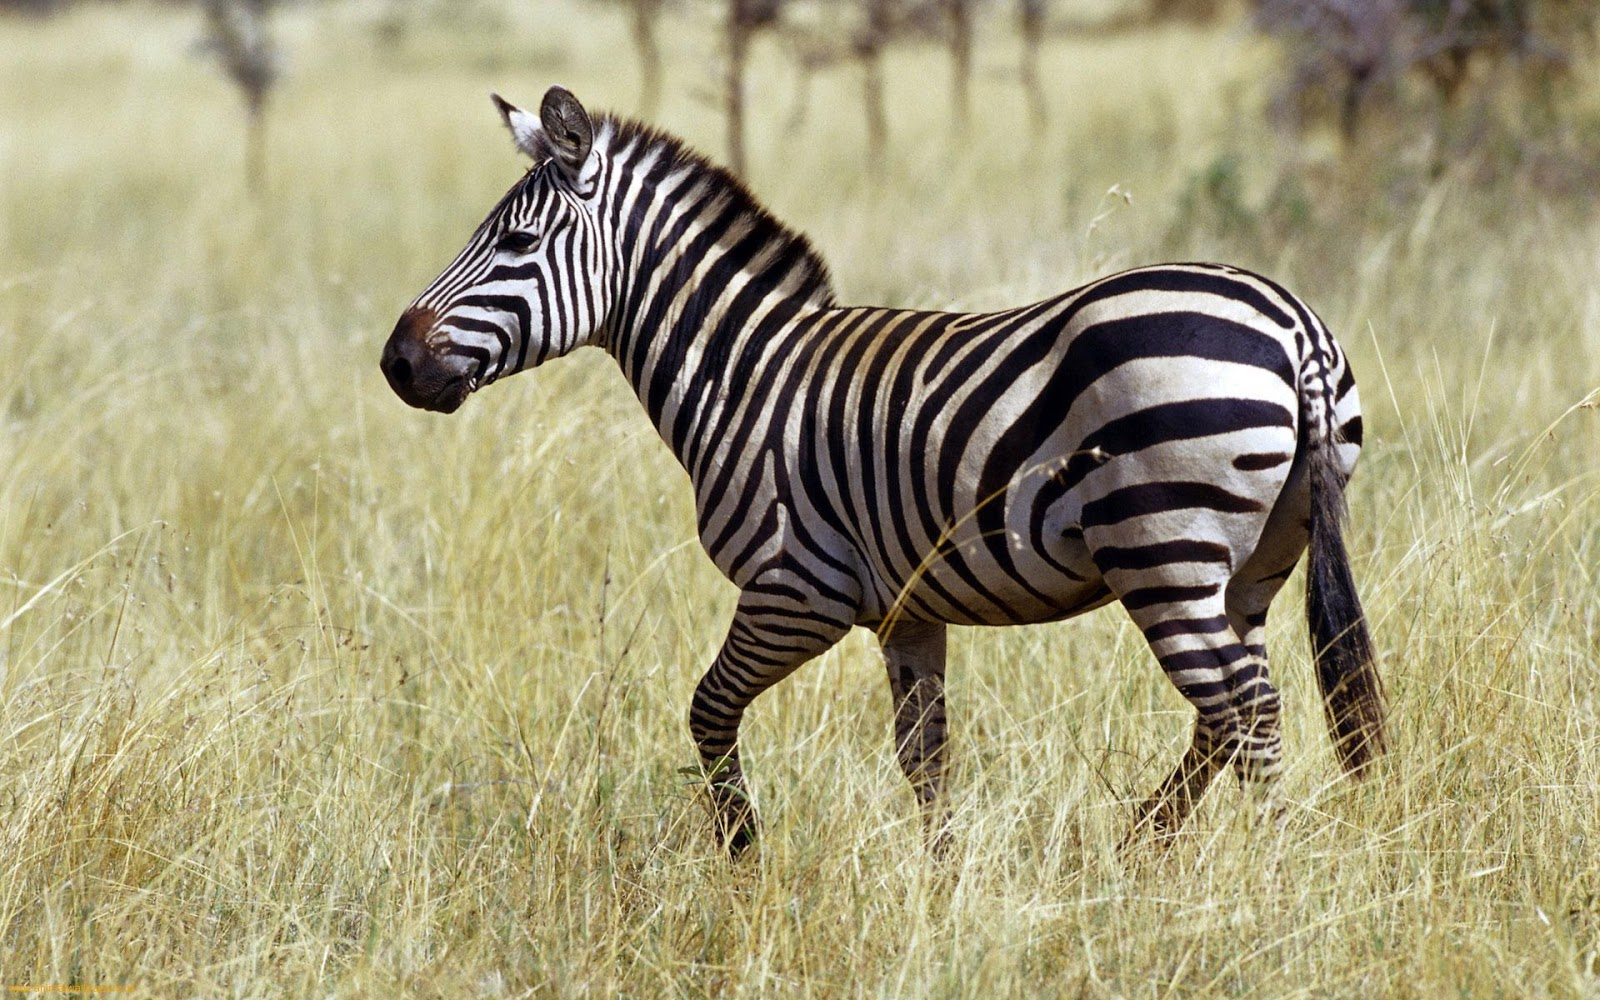
\includegraphics[width=\textwidth,height=1in]{figs/animal1}
        \caption{A Zebra}
        \label{fig:Zebra}
    \end{subfigure}
    ~ %add desired spacing between images, e. g. ~, \quad, \qquad, \hfill etc. 
      %(or a blank line to force the subfigure onto a new line)
    \begin{subfigure}[b]{0.3\textwidth}
        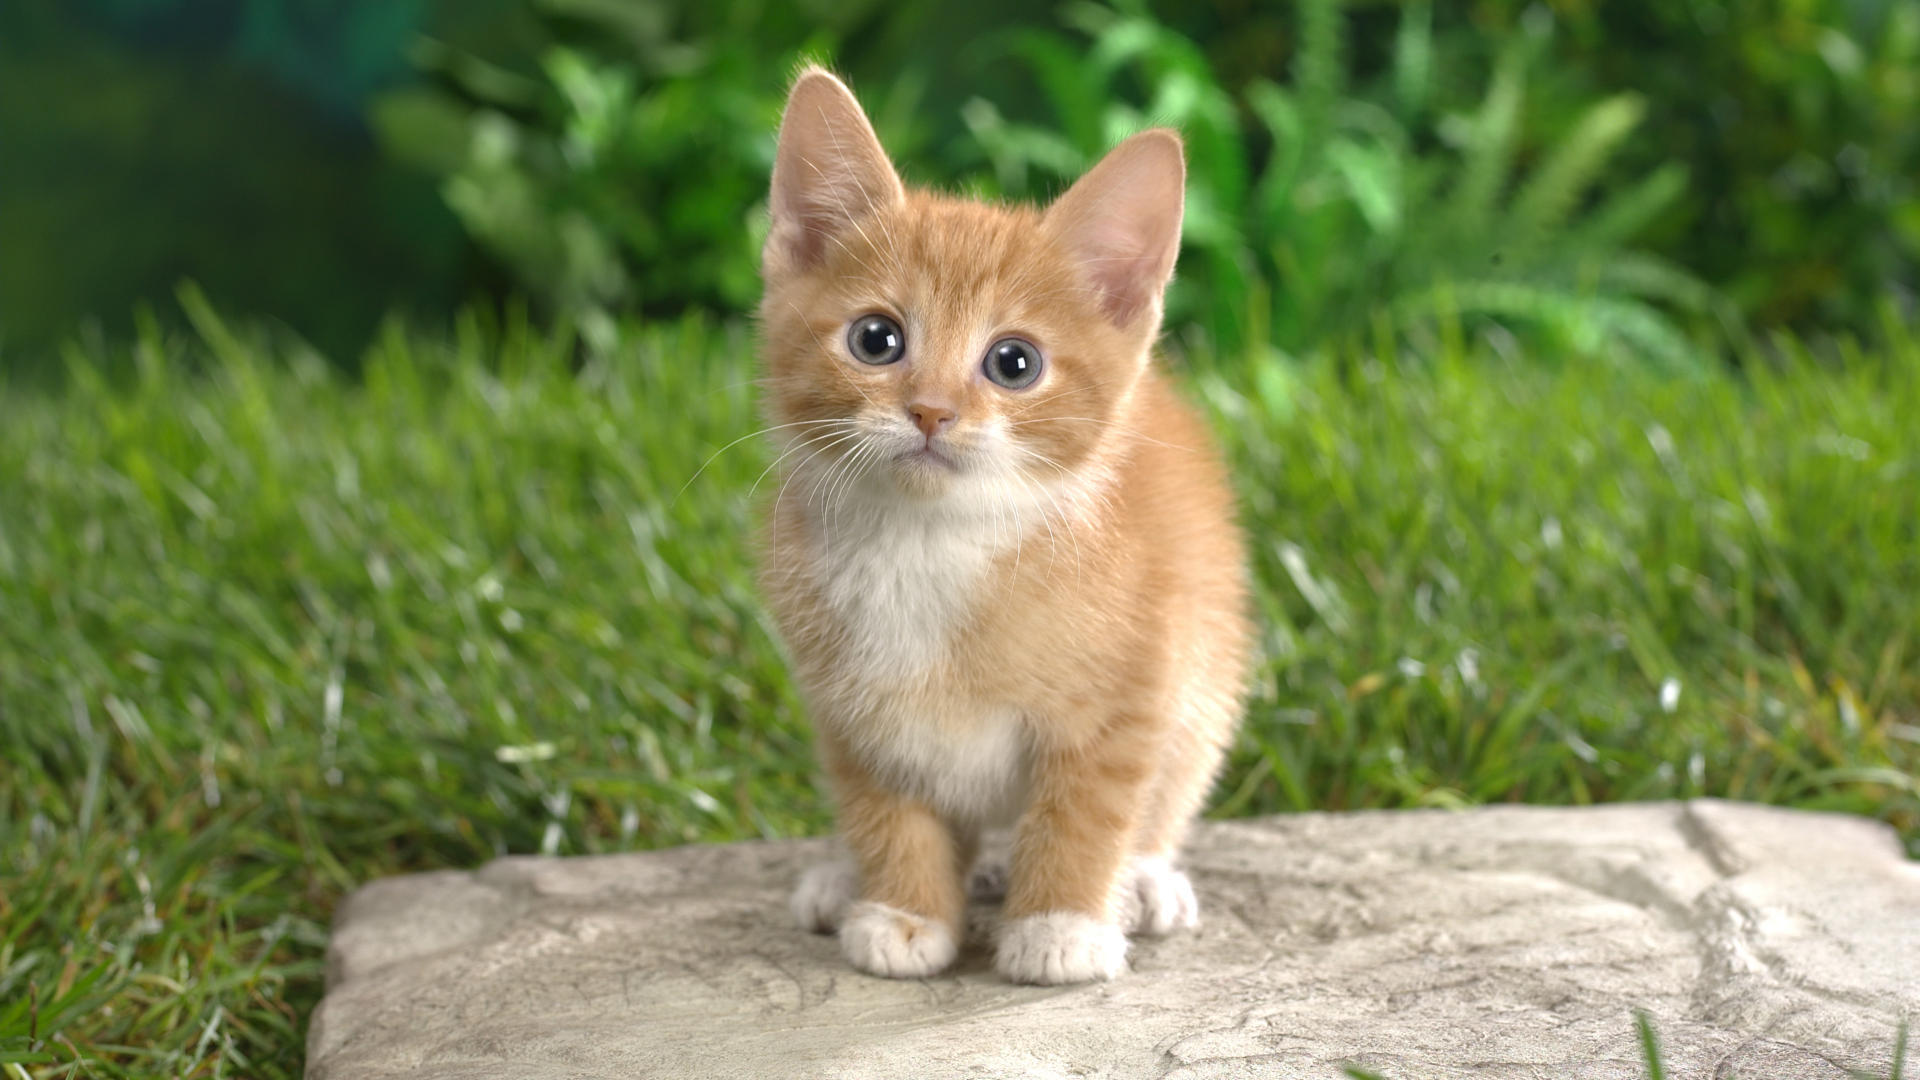
\includegraphics[width=\textwidth,height=1in]{figs/animal2}
        \caption{A Cat}
        \label{fig:cat}
    \end{subfigure}
    ~ %add desired spacing between images, e. g. ~, \quad, \qquad, \hfill etc. 
    %(or a blank line to force the subfigure onto a new line)
    \begin{subfigure}[b]{0.3\textwidth}
        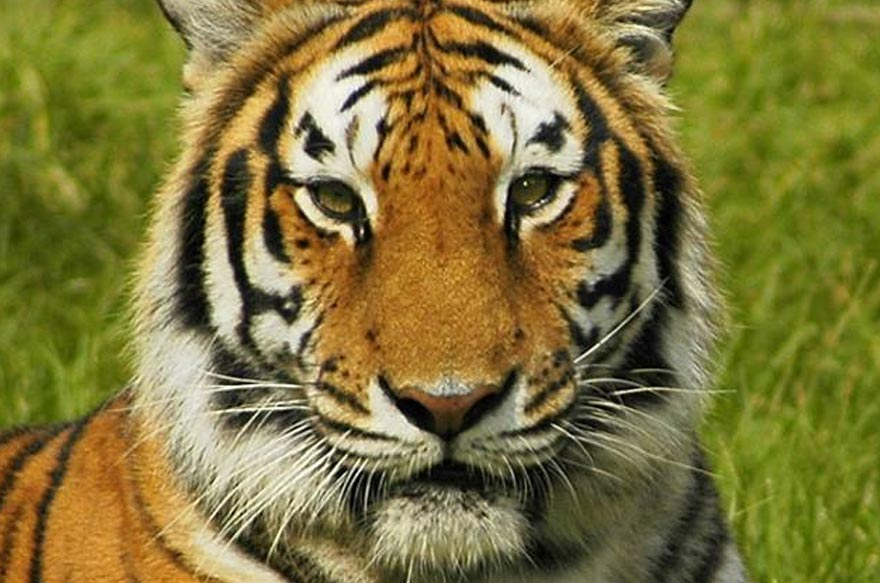
\includegraphics[width=\textwidth,height=1in]{figs/animal3}
        \caption{A Tiger}
        \label{fig:tiger}
    \end{subfigure}
    \caption{Pictures of animals}\label{fig:animals}
\end{figure}
\end{frame}
%%%%%%%%%%%%%%%%%%%%%%%%%%%%%%%%%%%%%%%%%%%%%%%%%%%%%%%%%%%%%%%%%%%%%%%%%%%%%%%%%%%%%%%%%%%%%%%%%%
\section[Structure]{Structuring a Presentation: Columns, Spaces \& Alignments}
\subsection{}
\begin{frame}[fragile]
  \frametitle{Using columns}
  \begin{footnotesize}
  
  \begin{verbatim}
  \begin{columns}
  \begin{column}{.5\textwidth}
\begin{block}{Block 1}
Block 1 text
\end{block}
  \end{column}
  \begin{column}{.5\textwidth}
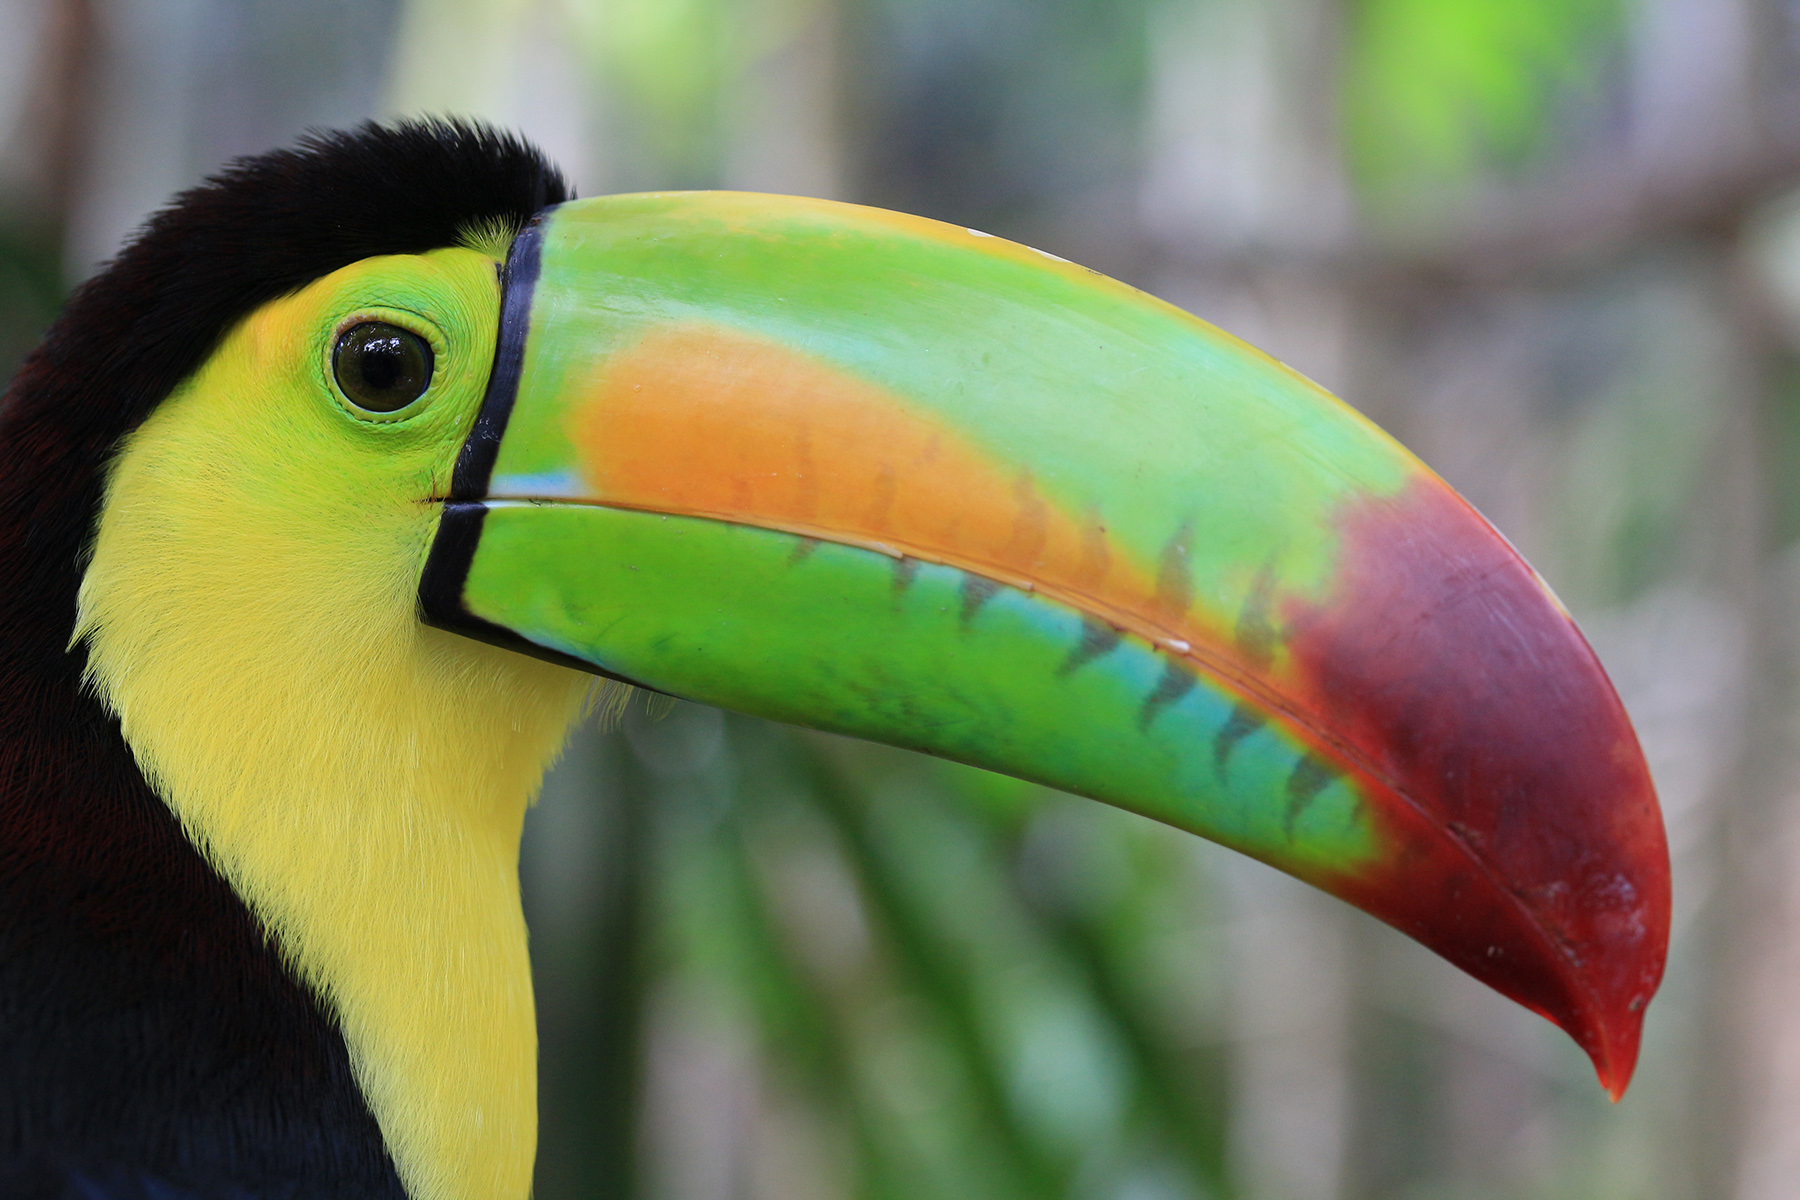
\includegraphics[height=1in]{figs/sample1}
  \end{column}
\end{columns}
\end{verbatim}
  \begin{columns}
  \begin{column}{.5\textwidth}
\begin{block}{Block 1}
Block 1 text
\end{block}
  \end{column}
  \begin{column}{.5\textwidth}
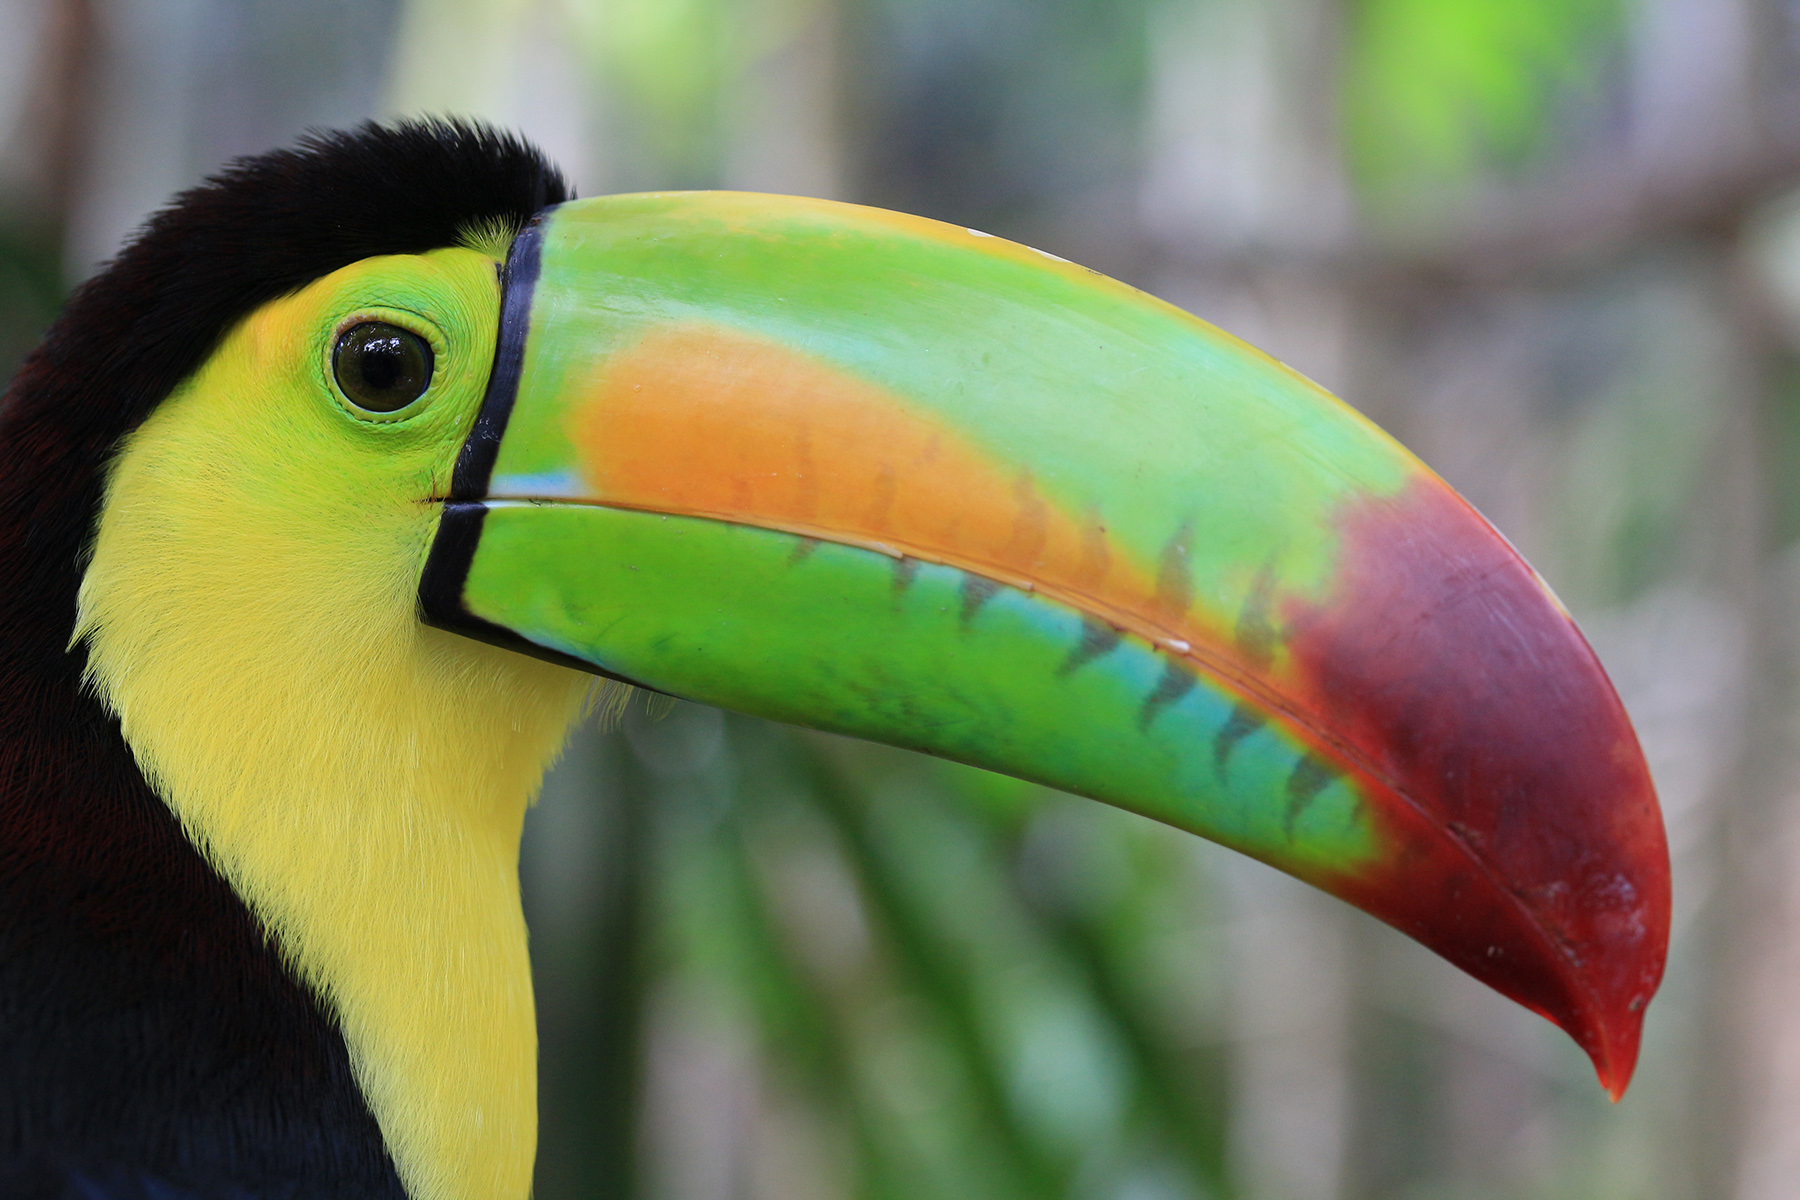
\includegraphics[height=1in]{figs/sample1}
  \end{column}
\end{columns}
  \end{footnotesize}
\end{frame}
%%%%%%%%%%%%%%%%%%%%%%%%%%%%%%%%%%%%%%%%%%%%%%%%%%%%%%%%%%%%%%%%%%%%%%%%%%%%%%%%%%%%%%%%%%%%%%%%%%
\subsection{}
\begin{frame}[fragile]
  \frametitle{Using minipage}
  \begin{verbatim}
  \begin{minipage}{.5\textwidth}
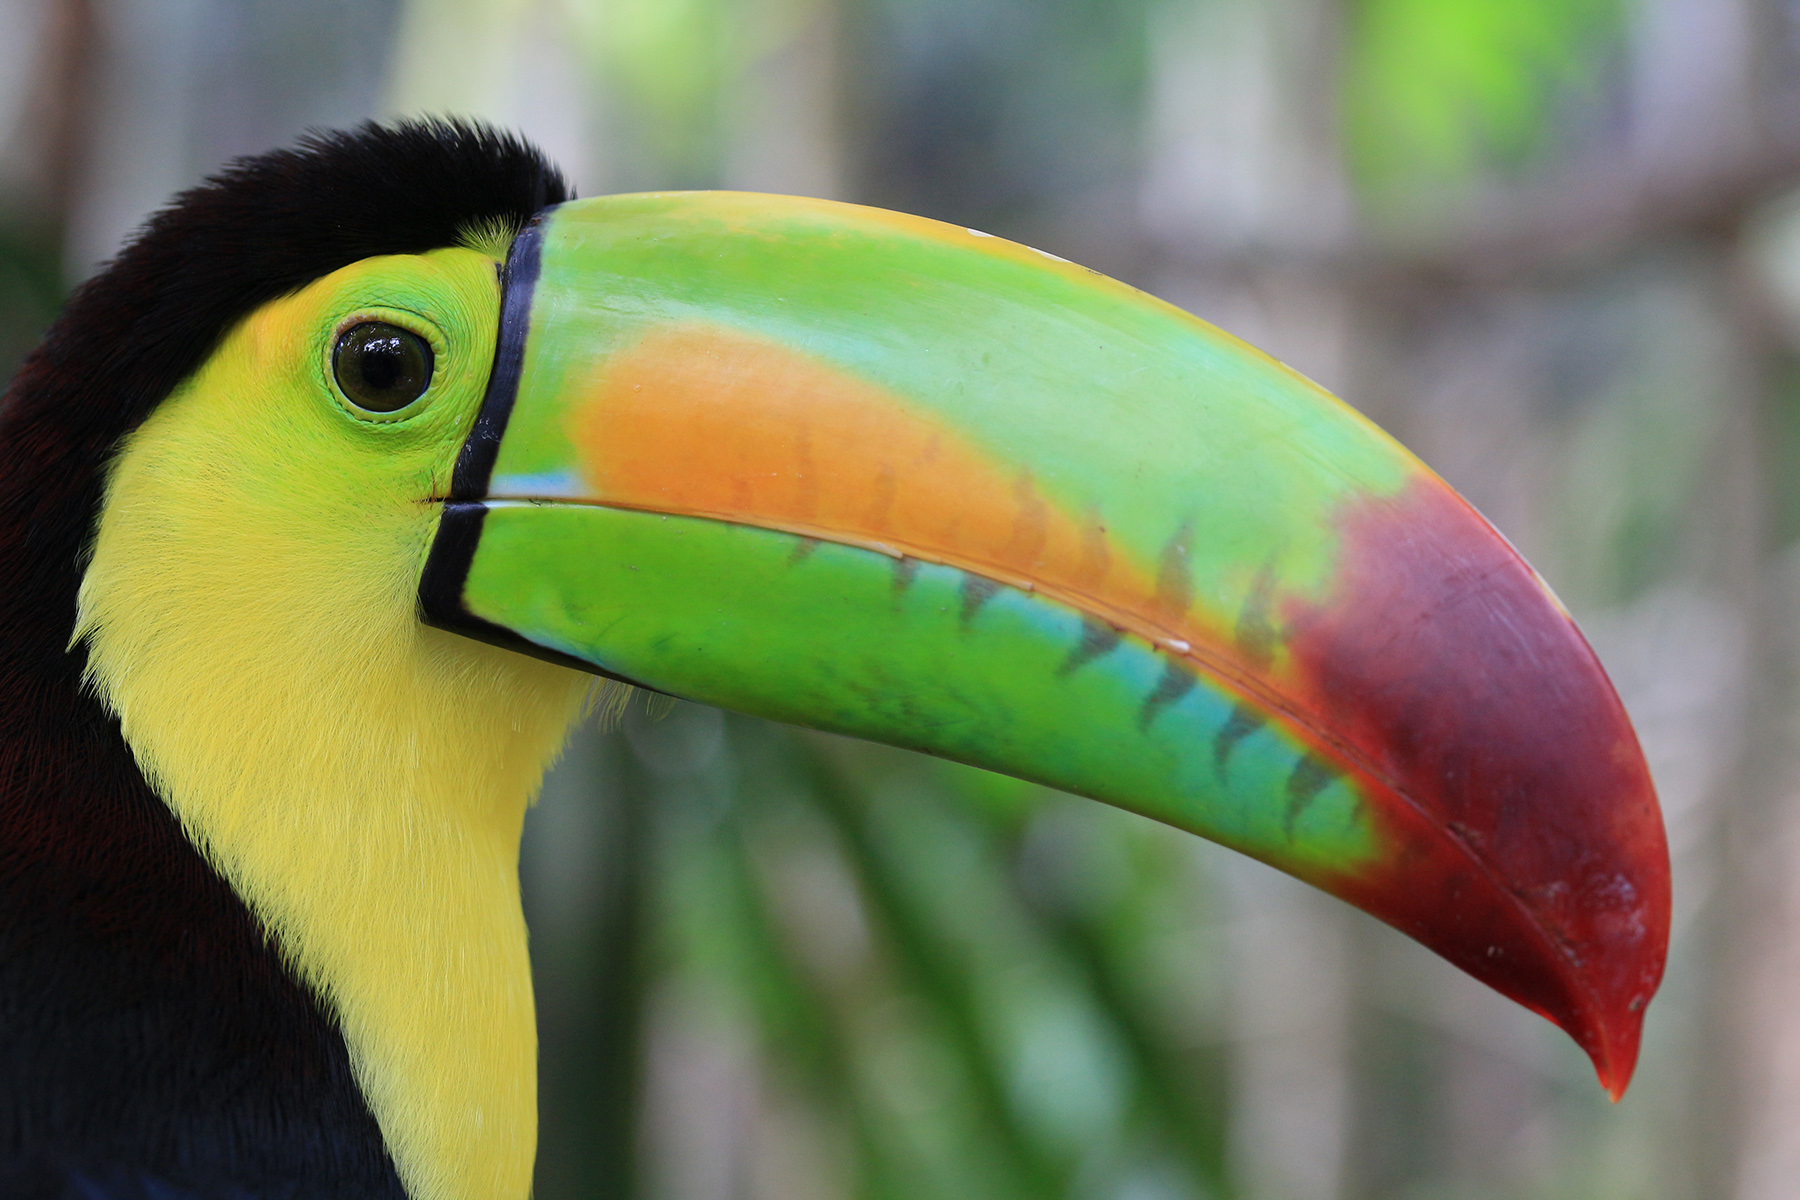
\includegraphics[height=1.in]{figs/sample1}
  \end{minipage}
  \hfill
  \begin{minipage}{.45\textwidth}
sample text sample text sample text
sample text sample text sample text
  \end{minipage}
  \end{verbatim}
  \begin{minipage}{.5\textwidth}
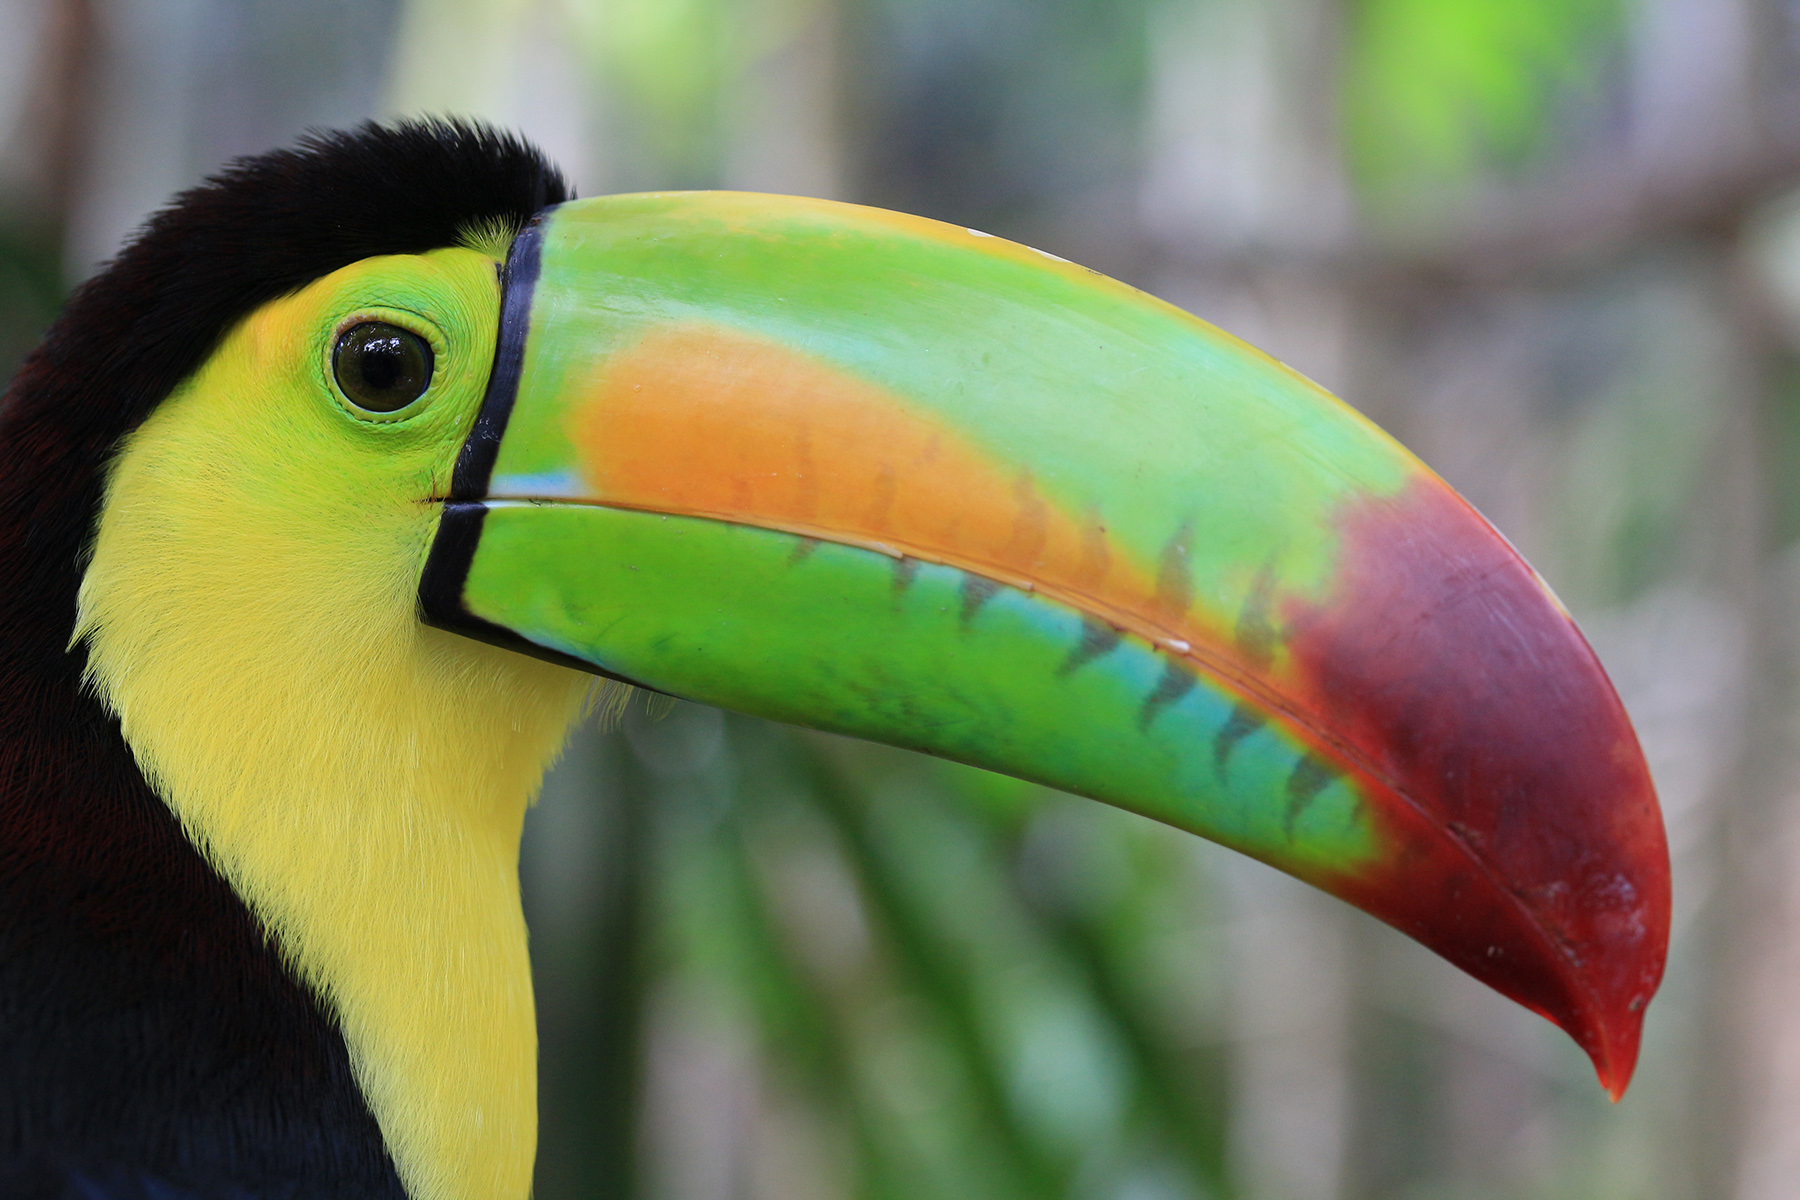
\includegraphics[height=1.in]{figs/sample1}
  \end{minipage}
  \hfill
  \begin{minipage}{.45\textwidth}
sample text sample text sample text
sample text sample text sample text
  \end{minipage}
\end{frame}
%%%%%%%%%%%%%%%%%%%%%%%%%%%%%%%%%%%%%%%%%%%%%%%%%%%%%%%%%%%%%%%%%%%%%%%%%%%%%%%%%%%%%%%%%%%%%%%%%%
\subsection{}
\begin{frame}[fragile]
  \frametitle{Alignments \& Spacings}
\begin{itemize}
  \item A frame can be assigned a left, center, or right alignment with the
flushleft, center and flushright environments
\end{itemize}
\begin{verbatim}
\begin{center}
The center aligned text goes here.
\end{center}
\end{verbatim}
\begin{block}{Centre aligned Example}
\begin{center}
The center aligned text goes here.
\end{center}
\end{block}
\begin{itemize}
  \item A vertical or horizontal space can be indicated by using \verb+\vspace{0.5cm}+ and \verb+\hspace{0.5cm}+, respectively.
\item Several units can be used, e.g, mm, cm, in, pt, ...
\item Also negative values can be used to squeeze text or graphics together: \verb+\vspace{-0.5cm}+
\end{itemize}
\end{frame}
%%%%%%%%%%%%%%%%%%%%%%%%%%%%%%%%%%%%%%%%%%%%%%%%%%%%%%%%%%%%%%%%%%%%%%%%%%%%%%%%%%%%%%%%%%%%%%%%%%
\section{Tables}
\subsection{}
\begin{frame}[fragile]
  \frametitle{Table Creation}
  \begin{flushleft}
  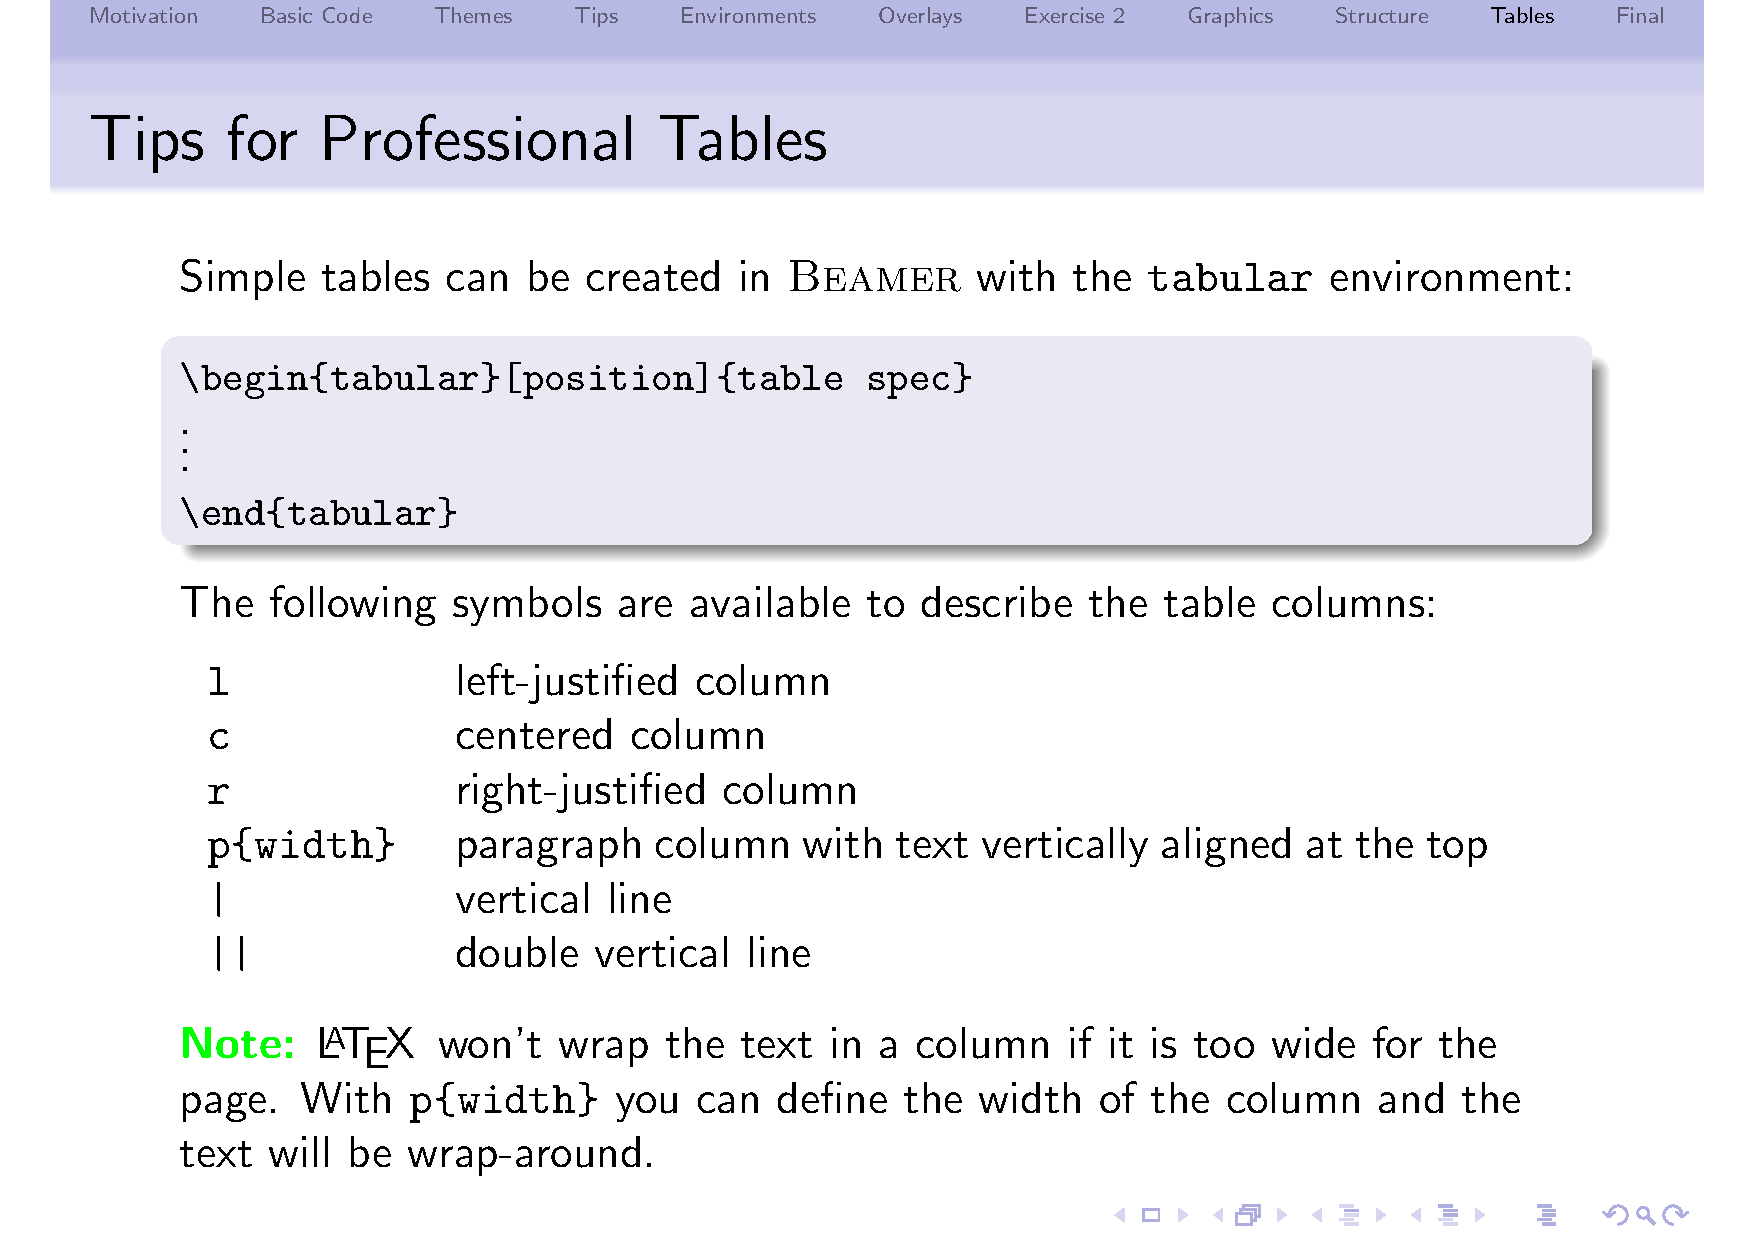
\includegraphics[scale=0.41]{figs/table}
  \end{flushleft}
\end{frame}
%%%%%%%%%%%%%%%%%%%%%%%%%%%%%%%%%%%%%%%%%%%%%%%%%%%%%%%%%%%%%%%%%%%%%%%%%%%%%%%%%%%%%%%%%%%%%%%%%%
\subsection{}
\begin{frame}[fragile]
  \frametitle{Table Creation: Examples}
\begin{columns}
\begin{column}{.5\textwidth}
\begin{small}
\begin{verbatim}
\begin{tabular}{l|c|r}
\hline
label 1 & label 2 & label 3 \\
\hline\hline
cell 1 & cell 2 & cell 3 \\
cell 4 & cell 5 & cell 6 \\
\hline
\end{tabular}
\end{verbatim}
\end{small}
\end{column}
\begin{column}{.5\textwidth}
\begin{tabular}{l|c|r}
\hline
label 1 & label 2 & label 3 \\
\hline\hline
cell 1 & cell 2 & cell 3 \\
cell 4 & cell 5 & cell 6 \\
\hline
\end{tabular}
    \end{column}
  \end{columns}
\end{frame}
%%%%%%%%%%%%%%%%%%%%%%%%%%%%%%%%%%%%%%%%%%%%%%%%%%%%%%%%%%%%%%%%%%%%%%%%%%%%%%%%%%%%%%%%%%%%%%%%%%
\subsection{}
\begin{frame}[fragile]
  \frametitle{Table Creation: Examples}
  For more professional looking tables use the booktabs package:
E.g. it provides the commands \verb+\toprule, \midrule & \bottomrule.+
\begin{columns}
\begin{column}{.5\textwidth}
\begin{small}
\begin{verbatim}
\begin{tabular}{c|c|c}
\toprule
label 1 & label 2 & label 3 \\
\midrule
cell 1 & cell 2 & cell 3 \\
cell 4 & cell 5 & cell 6 \\
\bottomrule
\end{tabular}
\end{verbatim}
\end{small}
\end{column}
\begin{column}{.5\textwidth}
\begin{tabular}{c|c|c}
\toprule
label 1 & label 2 & label 3 \\
\midrule
cell 1 & cell 2 & cell 3 \\
cell 4 & cell 5 & cell 6 \\
\bottomrule
\end{tabular}
    \end{column}
  \end{columns}
\end{frame}
%%%%%%%%%%%%%%%%%%%%%%%%%%%%%%%%%%%%%%%%%%%%%%%%%%%%%%%%%
%%%%%%%%%%%%%%%%%%%%%%%%%%%%%%%%%%%%%%%%%%%%%%%%%%%%%%%%%%%%%%%%%%%%%%%%%%%%%%%%%%%%%%%%%%%%%%%%%%
\fi
\subsection{}
\begin{frame}
  \frametitle{References}
\begin{block}{}
\begin{scriptsize}
\begin{thebibliography}{30}
\bibitem{beamer1}
Beamer Class:\\ \url{http://sourceforge.net/projects/latex-beamer/}
\bibitem{beamer2}
Beamer User Guide:\\
\url{http://ctan.imsc.res.in/macros/latex/contrib/beamer/doc/beameruserguide.pdf}
\bibitem{beamer3}
\LaTeX~ - beamer Course:
\url{http://impact.byu.edu/computation_seminar/latex/beamer-script.pdf}
\bibitem{beamer4}
{\color{red}For more model \LaTeX~ Files and Ebooks:
\url{https://bduportal.wordpress.com/latex/}}
\end{thebibliography}
\end{scriptsize}
\end{block}

\end{frame}
\usebackgroundtemplate{
\includegraphics[width=\paperwidth,height=\paperheight]{figs/thank-you.jpg}}
\begin{frame}[plain]
\vspace{4.35cm}
\begin{center}
\textbf{\color{green} {\Large www.idaravinthan.info}}
\end{center}
\end{frame}
\end{document}
\subsection{}
\begin{frame}[plain]
\textbf{\begin{center}
{\Huge Thank You.}
\end{center}}
\vfill
\vspace{2cm}
\begin{flushright}
Website: https://idaravinthan.info/
\end{flushright}
\end{frame}
\end{document}
%%%%%%%%%%%%%%%%%%%%%%%%%%%%%%%%%%%%%%%%%%%%%%%%%%%%%%%%%

\end{document}
